% Track-changes version of the manuscript, generated with latexdiff.
%   old: submission/GRH Paper/main.tex  (the version the reviewers read)
%   new: main.tex                       (current revision)
% Regenerate with:
%   latexdiff --append-textcmd="abstract" old.tex new.tex > main-diff.tex
% Red strikethrough = removed, blue underline = added.
%
% The Wiley class loads ulem without options; latexdiff needs normalem.
% Passing it globally here avoids an option clash.
\PassOptionsToPackage{normalem}{ulem}
\documentclass[MLA,Times1COL, hidelinks, doublespace]{WileyNJDv5} %STIX1COL,STIX2COL,STIXSMALL
%DIF LATEXDIFF DIFFERENCE FILE
%DIF DEL submission/GRH Paper/main.tex   Thu Aug  6 22:57:58 2026
%DIF ADD main.tex                        Wed Aug 12 10:13:36 2026
\usepackage{lineno}
\usepackage{amsmath}

%DIF 5a5
\graphicspath{{figures/}} %DIF > 
%DIF -------

\linenumbers

\articletype{Research Article}%

\received{Date Month Year}
\revised{Date Month Year}
\accepted{Date Month Year}
\journal{Journal}
\volume{00}
\copyyear{2023}
\startpage{1}

\raggedbottom
%DIF PREAMBLE EXTENSION ADDED BY LATEXDIFF
%DIF UNDERLINE PREAMBLE %DIF PREAMBLE
\RequirePackage[normalem]{ulem} %DIF PREAMBLE
\RequirePackage{color}\definecolor{RED}{rgb}{1,0,0}\definecolor{BLUE}{rgb}{0,0,1} %DIF PREAMBLE
\providecommand{\DIFadd}[1]{{\protect\color{blue}\uwave{#1}}} %DIF PREAMBLE
\providecommand{\DIFdel}[1]{{\protect\color{red}\sout{#1}}} %DIF PREAMBLE
%DIF SAFE PREAMBLE %DIF PREAMBLE
\providecommand{\DIFaddbegin}{} %DIF PREAMBLE
\providecommand{\DIFaddend}{} %DIF PREAMBLE
\providecommand{\DIFdelbegin}{} %DIF PREAMBLE
\providecommand{\DIFdelend}{} %DIF PREAMBLE
\providecommand{\DIFmodbegin}{} %DIF PREAMBLE
\providecommand{\DIFmodend}{} %DIF PREAMBLE
%DIF FLOATSAFE PREAMBLE %DIF PREAMBLE
\providecommand{\DIFaddFL}[1]{\DIFadd{#1}} %DIF PREAMBLE
\providecommand{\DIFdelFL}[1]{\DIFdel{#1}} %DIF PREAMBLE
\providecommand{\DIFaddbeginFL}{} %DIF PREAMBLE
\providecommand{\DIFaddendFL}{} %DIF PREAMBLE
\providecommand{\DIFdelbeginFL}{} %DIF PREAMBLE
\providecommand{\DIFdelendFL}{} %DIF PREAMBLE
%DIF AMSMATHULEM PREAMBLE %DIF PREAMBLE
\makeatletter %DIF PREAMBLE
\let\sout@orig\sout %DIF PREAMBLE
\renewcommand{\sout}[1]{\ifmmode\text{\sout@orig{\ensuremath{#1}}}\else\sout@orig{#1}\fi} %DIF PREAMBLE
\makeatother %DIF PREAMBLE
%DIF COLORLISTINGS PREAMBLE %DIF PREAMBLE
\RequirePackage{listings} %DIF PREAMBLE
\RequirePackage{color} %DIF PREAMBLE
\lstdefinelanguage{DIFcode}{ %DIF PREAMBLE
%DIF DIFCODE_UNDERLINE %DIF PREAMBLE
  moredelim=[il][\color{red}\sout]{\%DIF\ <\ }, %DIF PREAMBLE
  moredelim=[il][\color{blue}\uwave]{\%DIF\ >\ } %DIF PREAMBLE
} %DIF PREAMBLE
\lstdefinestyle{DIFverbatimstyle}{ %DIF PREAMBLE
	language=DIFcode, %DIF PREAMBLE
	basicstyle=\ttfamily, %DIF PREAMBLE
	columns=fullflexible, %DIF PREAMBLE
	keepspaces=true %DIF PREAMBLE
} %DIF PREAMBLE
\lstnewenvironment{DIFverbatim}[1][]{\lstset{style=DIFverbatimstyle}}{} %DIF PREAMBLE
\lstnewenvironment{DIFverbatim*}[1][]{\lstset{style=DIFverbatimstyle,showspaces=true}}{} %DIF PREAMBLE
\lstset{extendedchars=\true,inputencoding=utf8}

%DIF END PREAMBLE EXTENSION ADDED BY LATEXDIFF

\begin{document}

\title{A \DIFdelbegin \DIFdel{real time }\DIFdelend \DIFaddbegin \DIFadd{real-time }\DIFaddend reservoir inflow forecast evaluation framework}

\author[1]{Cameron Bracken}
\author[1]{Youngjun Son}
\author[1]{Vince Tidwell}
\author[1]{Nathalie Voisin}

\authormark{BRACKEN \textsc{et al.}}
\titlemark{xxx}

\address[1]{\orgname{Pacific Northwest National Laboratory}, \orgaddress{\state{Washington}, \country{USA}}}

\corres{Corresponding author Cameron Bracken, \email{cameron.bracken@pnnl.gov}}

%\presentaddress{This is sample for present address text this is sample for present address text.}

%\fundingInfo{Text}
%\JELinfo{ejlje}

\abstract[Abstract]{
Recent advances in data driven hydrologic forecasts have led to a multitude of new and rapidly improving streamflow forecast products and technologies. These often lead hydropower producers to question whether such advances translate into increases in revenue and whether implementing these new forecasts justify the additional associated costs. To address this, we present a general framework that can be used in real time (or near real time) for reservoir inflow forecast evaluation. The \DIFaddbegin \DIFadd{goal of this }\DIFaddend framework \DIFdelbegin \DIFdel{calls }\DIFdelend \DIFaddbegin \DIFadd{is to provide hydropower operators and water managers with information necessary }\DIFaddend for \DIFdelbegin \DIFdel{an iterative approach which involves direct operator feedback }\DIFdelend \DIFaddbegin \DIFadd{evaluating how much a particular forecast product will improve their operations and ultimately inform ongoing investment or development decisions, such as whether to purchase external forecast products or improve existing internal forecasting capabilities. In our framework, operators participate }\DIFaddend in \DIFaddbegin \DIFadd{designing }\DIFaddend the \DIFaddbegin \DIFadd{metrics and the }\DIFaddend evaluation \DIFdelbegin \DIFdel{process}\DIFdelend \DIFaddbegin \DIFadd{runs using the same operational data the operators use}\DIFaddend . The evaluation can include forecast verification and validation, but also includes other qualitative or specialized metrics of forecast quality\DIFaddbegin \DIFadd{, differentiating it from a standard retrospective forecast verification}\DIFaddend . We \DIFdelbegin \DIFdel{also }\DIFdelend present \DIFdelbegin \DIFdel{a successful }\DIFdelend \DIFaddbegin \DIFadd{an }\DIFaddend application of this evaluation framework to three reservoirs in the Great River Hydro system on the Connecticut River in the Northeast U.S.\DIFaddbegin \DIFadd{, where a metric tailored to assess regulatory compliance risk helped distinguish between forecast products where standard metrics could not. }\DIFaddend While there is no single evaluation approach that can apply to all hydrologic forecasts, we also present a range of options of both traditional and tailored metrics that \DIFdelbegin \DIFdel{will be }\DIFdelend \DIFaddbegin \DIFadd{are }\DIFaddend suitable for a diverse set of situations and systems.
\DIFdelbegin \DIFdel{The goal of this framework is to provide hydropower operators with information necessary for evaluating how much a particular forecast product will improve their operations and ultimately inform ongoing investment decisions, such as whether to purchase external forecast products or improve existing internal forecasting capabilities.
}\DIFdelend }

\DIFdelbegin %DIFDELCMD < \keywords{hydropower, streamflow forecasting, real time evaluation, verification, validation}
%DIFDELCMD < %%%
\DIFdelend \DIFaddbegin \keywords{hydropower, streamflow forecasting, real-time evaluation, verification, validation}
\DIFaddend 

%\jnlcitation{\cname{%
%\author{Walters G}, and
%\author{Bracken C}}.
%\ctitle{A comprehensive calibration approach for the Northwest River Forecast Center} \cjournal{\it JAWRA} \cvol{2021;00(00):1--18}.}


\maketitle

%\section{Highlights}
%1) More inflow forecasts products are becoming available to hydropower operators
%2) The forecast verification exercise transitions from “value of forecasts” to “added value of better forecasts”. 
%3) The operators are critical to develop the periods and metrics to define the "added value".
%4)	While hindcasts provide robust statistics, operators tend to favor a shorter evaluation period under real time operational conditions



\section{Introduction}

%i)	Role of forecasts in hydropower scheduling
%ii)	Improvements and uncertainties in forecasts
%iii)	Question of whether fidelity of forecasts can improve scheduling and thus need of tailored evaluation
%iv)	Objective: Demonstrate forecast evaluation process 
%v)	Brief description of approach 

Changing environmental regulation, diversifying and increasing water demands, and growing operational uncertainties are requiring more precise operations of reservoir and hydropower systems (e.g., \cite{leeDevelopingResilientReservoir2025,guoReservoirControlOperations2024,badrDamSystemReservoir2023,aljodaUncertaintiesRisksReservoir2021}). This desire for increased precision has driven interest in improved streamflow forecasting tools \citep{yangSensitivityForecastValue2021,paganoChallengesOperationalRiver2014, liuAdvancingDataAssimilation2012}. While numerous commercial and in-house options are available, water managers are faced with the challenge of evaluating whether more sophisticated forecasting tools will actually improve their operations and justify the associated financial investment. 

%<I would also add here that we see more forecast products coming in with new optimization and new data driven approaches - however old approaches for forecast verification  might be outdated - those need to be evaluated on context on needing the perturb an existing system. Many papers on LSTM and stuff currently say that they develop real time models. This study provides insight to this technology innovation on how to evaluate their value.>

The quality of hydrologic forecasts and hydropower scheduling has rapidly improved in recent years due to the emergence of new data driven approaches \DIFdelbegin \DIFdel{\mbox{%DIFAUXCMD
\citep{kratzertLearningUniversalRegional2019} }\hskip0pt%DIFAUXCMD
}\DIFdelend \DIFaddbegin \DIFadd{\mbox{%DIFAUXCMD
\citep{kratzertLearningUniversalRegional2019a} }\hskip0pt%DIFAUXCMD
}\DIFaddend and scheduling optimization \citep{zhangOptimizationShorttermHydropower2024}. Despite \DIFdelbegin \DIFdel{these improvements verification remains a challenge and traditional verification approaches may not be applicable under new operational paradigms. This study seeks to provide insight into the evaluation of contemporary forecast models and guidance on how to assess their value}\DIFdelend \DIFaddbegin \DIFadd{this, the practice of forecast verification has remained mostly unchanged. A traditional forecast verification requires evaluation of hindcasts using standard statistical metrics, over a period which is representative of the full climatological record, often 30 years or more. The high cost of hindcasts and strict data requirements are two reasons full verifications are not done in practice. The second best approach, if hindcasts are not available, is to evaluate archived operational forecasts, although this approach fits poorly with products that are updated continuously, trained on evolving data streams, hand adjusted by operators, or developed by third parties. The gap this study addresses is to develop a procedure by which hydropower or reservoir operators can evaluate forecasts on their own system under familiar operating conditions}\DIFaddend .

Pairing a forecasting tool with the needs of a particular \DIFdelbegin \DIFdel{hydropower }\DIFdelend operator is complicated by a number of factors. The quantity and quality of data concerning meteorological (precipitation, snow pack) and hydrological (reservoir storage, soil moisture) conditions within the watershed vary locationally as do the efficacy of meteorological forecasting (Hay et al. 2023; Chen et al. 2021; Wood et al. 2016). Watershed characteristics vary as does the infrastructure used to manage basin resources \citep{phamEvaluationRandomForests2021}. Operators are often subject to very different management regimes (e.g., run-of-river, rule curves) \citep{zajacImpactLakeReservoir2017}. Management objectives also vary according to forecast lead time as well as normal versus extreme event conditions. Additionally, there are decisions concerning choice of model (conceptual, physical, empirical, AI enhanced) as well as its calibration and parameterization.  

To help provide some clarity concerning the performance of various forecasting tools under differing informational, physical, and operational conditions, a range of head-to-head evaluation exercises have been performed. HEPEX (which stands for Hydrologic Ensemble Prediction EXperiment), which “seeks to advance the science and practice of hydrological ensemble prediction and its use in impact- and risk-based decision making,” has organized evaluations in the context of community experiments and testbeds (\footnote{\url{www.hepex.org}}). The U.S. Bureau of Reclamation has also performed a series of forecast rodeos in a prize competition environment\footnote{\url{https://www.usbr.gov/research/challenges/forecastrodeo.html}}. Real time forecast evaluations such as this (as opposed to retrospective evaluations) tend to be favored by the industry due their ability to fit in with existing operations \citep{krajewskiRealtimeStreamflowForecasting2021}. While such exercises provide valuable insight into the complexities and potential solutions for streamflow forecasting it doesn’t answer the question on operators’ minds—will a new forecast tool improve my operations enough to justify the investment in infrastructure, staff training and staff time during transition? 

Here we present an approach for assisting local water managers and hydropower utility operators in performing a context-specific evaluation of streamflow forecasting and hydropower scheduling tools. The approach calls for broad integration of the operator including experimental design, metric selection, tailored metric design, and comparative analysis \DIFaddbegin \DIFadd{and visualization }\DIFaddend of the results. \DIFaddbegin \DIFadd{The contribution of this work is a specific operating procedure for the case where a utility must choose between competing forecast products under live operating conditions and cannot run a hindcast. That procedure has two components that distinguish it from retrospective verification practice. First, the operators participate in metric selection and design and can modify, remove, or append metrics to the evaluation as more data is collected. Second, the evaluation runs on the same operational data the operators use which reflects the real day-to-day operational decisions. 
}

\DIFaddend We then demonstrate this approach in the context of three hydropower plants operated by Great River Hydro, the largest conventional hydropower provider in the Northeastern U.S. By using multiple traditional and tailored metrics as well as making the \DIFdelbegin \DIFdel{data }\DIFdelend \DIFaddbegin \DIFadd{forecast evaluation information }\DIFaddend easily accessible and comparable, this approach provides operators with the information they need to make informed decisions on forecast products\DIFdelbegin \DIFdel{with confidence}\DIFdelend . Importantly, this approach is designed to be easily replicated on other river systems.


\section{Methods}

%(1)	real time vs. historical
While probabilistic and ensemble forecasts and evaluation metrics are gaining in popularity, deterministic forecasts such as those issued by the National Weather Service River Forecast Centers (RFC) are still widely used operationally and are adopted as a \DIFdelbegin \DIFdel{valued benchmark of }\DIFdelend \DIFaddbegin \DIFadd{benchmark in }\DIFaddend this framework. \DIFaddbegin \DIFadd{All three products evaluated here are deterministic, so the metrics we describe are deterministic; Section \ref{sec:probabilistic} sets out how the framework extends to ensemble products, since the structure of the process does not depend on which kind of forecast is being evaluated. }\DIFaddend In addition, we focus on metrics which are feasible to compute in a \DIFdelbegin \DIFdel{real time }\DIFdelend \DIFaddbegin \DIFadd{real-time }\DIFaddend setting as opposed to a hindcast based evaluation. 
\DIFdelbegin \DIFdel{While a hindcast evaluation may be preferable statistically, hindcast evaluations require that forecasters predict (manually or with an operations model) their own behavior during hypothetical past conditionswhere other factors such as market pricesand data curation issues may not be known. }\DIFdelend \DIFaddbegin 

\DIFadd{Although they can be costly to produce, hindcasts are the most statistically robust way to evaluate a particular forecast model. A hindcast evaluation of forecast quality does not itself require re-operating the system, since forecasts of inflow can be compared directly against observed or calculated inflow. Yet, two complications arise in this setting. First, where the forecast is modified using human judgment, a hindcast requires forecasters to reconstruct the decisions they would have made under past conditions. Those conditions may include electricity prices, weather conditions, or other operational conditions that may be difficult to reconstruct after the fact. Second, extending the evaluation from forecast quality to forecast value (e.g., streamflow to megawatts) requires a reservoir operations model or manual operator input. A real-time evaluation avoids both complications by developing a forecast archive over time and relying on real operator decisions. }\DIFaddend In the remainder of this section we describe the components of a \DIFdelbegin \DIFdel{real time }\DIFdelend \DIFaddbegin \DIFadd{real-time }\DIFaddend forecast evaluation framework for reservoir inflow forecasts including visualizations to convey the evaluation results and an iterative feedback process from the operators.
%are onerous to conduct in humapn-in-the-loop forecaster settings. 
%are often not possible in operational settings due to forecaster time constratrain
%Note for self to work on: the intro needs more context on how it informs the community. Real time is definitely good. papers such as : https://www.sciencedirect.com/science/article/pii/S2589915521000389 could help make the case 

\subsection{\DIFdelbegin \DIFdel{real time }\DIFdelend \DIFaddbegin \DIFadd{Real-time }\DIFaddend inflow forecast evaluation\DIFdelbegin %DIFDELCMD < \MBLOCKRIGHTBRACE
%DIFDELCMD < %%%
\DIFdel{A general real time }\DIFdelend \DIFaddbegin }\label{sec:realtime}
\DIFadd{A general real-time }\DIFaddend forecast evaluation process can be described in the following steps\DIFdelbegin \DIFdel{:
}\DIFdelend \DIFaddbegin \DIFadd{. Steps 1 through 3 are generic practice, common to any verification exercise. Steps 4 through 6 are where this framework departs from retrospective verification.
}\DIFaddend \begin{enumerate}
    \item \textbf{Collect \DIFdelbegin \DIFdel{real time }\DIFdelend \DIFaddbegin \DIFadd{real-time }\DIFaddend data} - This may include streamflow forecasts (natural or regulated), calculated inflows, scheduled and actual outflows, and other data relevant for computing evaluation-relevant metrics such as forecast issue times and past forecasts.
    \item \textbf{Compute evaluation metrics} - At the start of an evaluation, it may only be possible to compute a limited number of generic evaluation metrics but as the available data grows it may become possible to compute more reliable metrics as well as metrics tailored to the specific system.
    \item \textbf{Visualization} - Developing easy to interpret visuals is critical to the success of an evaluation. Visuals should be concise, clear, and require a limited amount of explanation, or come with built-in documentation.
    \item \textbf{\DIFdelbegin \DIFdel{Solicit }\DIFdelend \DIFaddbegin \DIFadd{Gather }\DIFaddend feedback} - Collecting feedback on an ongoing basis from operators is critical to the success of a \DIFdelbegin \DIFdel{real time }\DIFdelend \DIFaddbegin \DIFadd{real-time }\DIFaddend forecast evaluation. \DIFdelbegin \DIFdel{This process can be used }\DIFdelend \DIFaddbegin \DIFadd{Operators should be asked which recent forecast errors mattered operationally and which did not, since the answers are not always apparent from the metrics alone.
    }\item \textbf{\DIFadd{Update metrics}} \DIFadd{- Feedback is used to add metrics tailored }\DIFaddend to \DIFdelbegin \DIFdel{develop tailored metrics that are specific to }\DIFdelend the system or reservoir being evaluated\DIFdelbegin \DIFdel{. 
    }\DIFdelend \DIFaddbegin \DIFadd{, and to remove or modify metrics that have proven uninformative. The set of metrics is therefore not fixed at the outset but develops as the evaluation proceeds.
    }\DIFaddend \item \textbf{Iterate} - The above steps should be repeated at a regular interval (monthly or weekly) throughout the entire forecast evaluation period, ideally at least one year in duration.
\end{enumerate}

The \DIFdelbegin \DIFdel{iterative nature of this evaluation process with direct operator feedback is important to its success.
As more data becomes available so does an understanding of the forecast performance which may help to develop additional tailored metrics }\DIFdelend \DIFaddbegin \DIFadd{mechanics of steps 4 and 5 determine what the evaluation produces, so an example of how feedback was collected and acted on in our case helps clarify this point. Feedback was collected in recurring meetings with the operators, held monthly for most of the evaluation. Each meeting reviewed the current calculated metrics against recent operating experience, and operators were asked to identify which recent forecast errors mattered operationally, and which did not. The answers frequently diverged from what the generic metrics indicated, especially during the high-flow season. Operators discounted large errors during high-flow spill conditions, when they had little discretion over releases and forecast quality was operationally irrelevant, while treating moderate errors with the potential to impact the forebay compliance band as serious. These ongoing discussions motivated the tailored metrics in Section \ref{sec:tailored}: the forebay exceedance metrics were designed in direct response to operators stating that compliance risk, rather than average error, determined whether they trusted a forecast.
}

\DIFadd{The iteration in step 6 involves two timescales that should not be conflated. Metric development was completed within roughly the first six months of our evaluation, after which the iteration served to accumulate data rather than to identify new metrics. A minimum defensible skill assessment requires at least one full annual cycle, since forecast performance may vary substantially by season (Section \ref{sec:seasonal}) and different forecast models may rank differently in each season. Operators should therefore expect the set of metrics to stabilize well before the evaluation period ends}\DIFaddend . The following sections detail some additional considerations \DIFdelbegin \DIFdel{.
}\DIFdelend \DIFaddbegin \DIFadd{when conducting a real-time forecast evaluation.
%DIF > We note a tension the operators raised: industry preference is for shorter evaluations, sometimes a single season, while a single season samples only one hydrologic outcome. The following sections detail some additional considerations.
}\DIFaddend 

%iii)	Benchmark
\subsection{Benchmark forecasts}\DIFdelbegin \DIFdel{It is critical to include benchmark forecasts in the evaluation }\DIFdelend \DIFaddbegin \label{sec:benchmarks}
\DIFadd{Benchmark forecasts of known quality }\DIFaddend to provide forecast evaluators with context for how well \DIFdelbegin \DIFdel{a specific forecast performs over the benchmarks.}\DIFdelend \DIFaddbegin \DIFadd{certain forecasts performs over a benchmark (a.k.a. reference) forecast. }\DIFaddend Two commonly used benchmarks are the ``perfect'' forecasts, which use observed or calculated inflows in place of a \DIFaddbegin \DIFadd{true }\DIFaddend forecast to get a sense of the best possible forecast, and ``persistence'' forecasts which use the last observed value carried out for all future timesteps\DIFdelbegin \DIFdel{to get a sense of the arguably worst possible forecast}\DIFdelend . Persistence is a \DIFdelbegin \DIFdel{competitive benchmark for short term operations}\DIFdelend \DIFaddbegin \DIFadd{simple but competitive forecast at short lead times}\DIFaddend , from hours to \DIFaddbegin \DIFadd{roughly two days, and is the appropriate reference for day-ahead operations, which is the horizon of interest for the system evaluated here. It degrades quickly beyond that horizon, where a climatological forecast is the more appropriate lower bound. Evaluators should match the benchmark to the horizon of interest: persistence for hourly to }\DIFaddend 2-day \DIFdelbegin \DIFdel{horizons. We note that other simple climatologically driven forecasts could be used in place of the persistence forecast when looking at longer horizons like monthly and seasons}\DIFdelend \DIFaddbegin \DIFadd{operations, climatology for weekly to seasonal horizons. Where persistence is plotted at longer lead times in the figures below, it is retained only to show the scale of degradation and should not be read as a meaningful reference at those horizons}\DIFaddend . Other benchmarks could include publicly available forecast products or any other forecast that is currently being used at the reservoir.

\DIFaddbegin \DIFadd{Reporting skill relative to a benchmark is also useful because NSE and KGE are referenced to the variance of the observations at each location, so their values are not directly comparable across locations with different inflow variability \mbox{%DIFAUXCMD
\citep{knobenTechnicalNoteInherent2019a}}\hskip0pt%DIFAUXCMD
. The NSE makes this concrete: it is itself a skill score measured against the mean of the observations, so an NSE value says how much a forecast improves on that particular reference and nothing more. Where the mean is a poor reference the same forecast will score higher than it will where the mean is already hard to beat, and comparing raw values across sites can therefore give a skewed ranking, an effect we demonstrate in Section \ref{sec:period}. We therefore recommend reporting skill scores relative to a deliberately chosen benchmark alongside the raw metrics in any multi-site evaluation.
}



\DIFaddend %(2)	Measured inflow (smoothing)  (Figure)
\subsection{Smoothing calculated inflows}
Most available reservoir inflow data is not directly measured, instead it is computed based on measured changes in forebay elevation and a known elevation-volume relationship. These calculations are often noisy due to short term fluctuations in forebay elevations from wind, turbine\DIFaddbegin \DIFadd{, }\DIFaddend and spillway release changes, \DIFdelbegin \DIFdel{and other such as reservoir seiches}\DIFdelend \DIFaddbegin \DIFadd{reservoir seiches, }\DIFaddend or waves propagating from upstream. Inflow computed in this way can often contain negative values and other non-physical fluctuations. In this situation we recommend the inflow data be smoothed prior to comparing with any forecasted inflow. We recommend a triangular smoother that applies moving-averages using a triangular weight function. This is a simple option which produces reasonable results but many more options are available \citep{elshorbagyNoiseReductionChaotic2002}. 
\DIFdelbegin \DIFdel{Figure \ref{fig:smoothing} shows an example of hourly computed inflow data which has been smoothed using a triangular smoother. 
}\DIFdelend 



\DIFdelbegin %DIFDELCMD < \begin{figure}
%DIFDELCMD <     \centering
%DIFDELCMD <     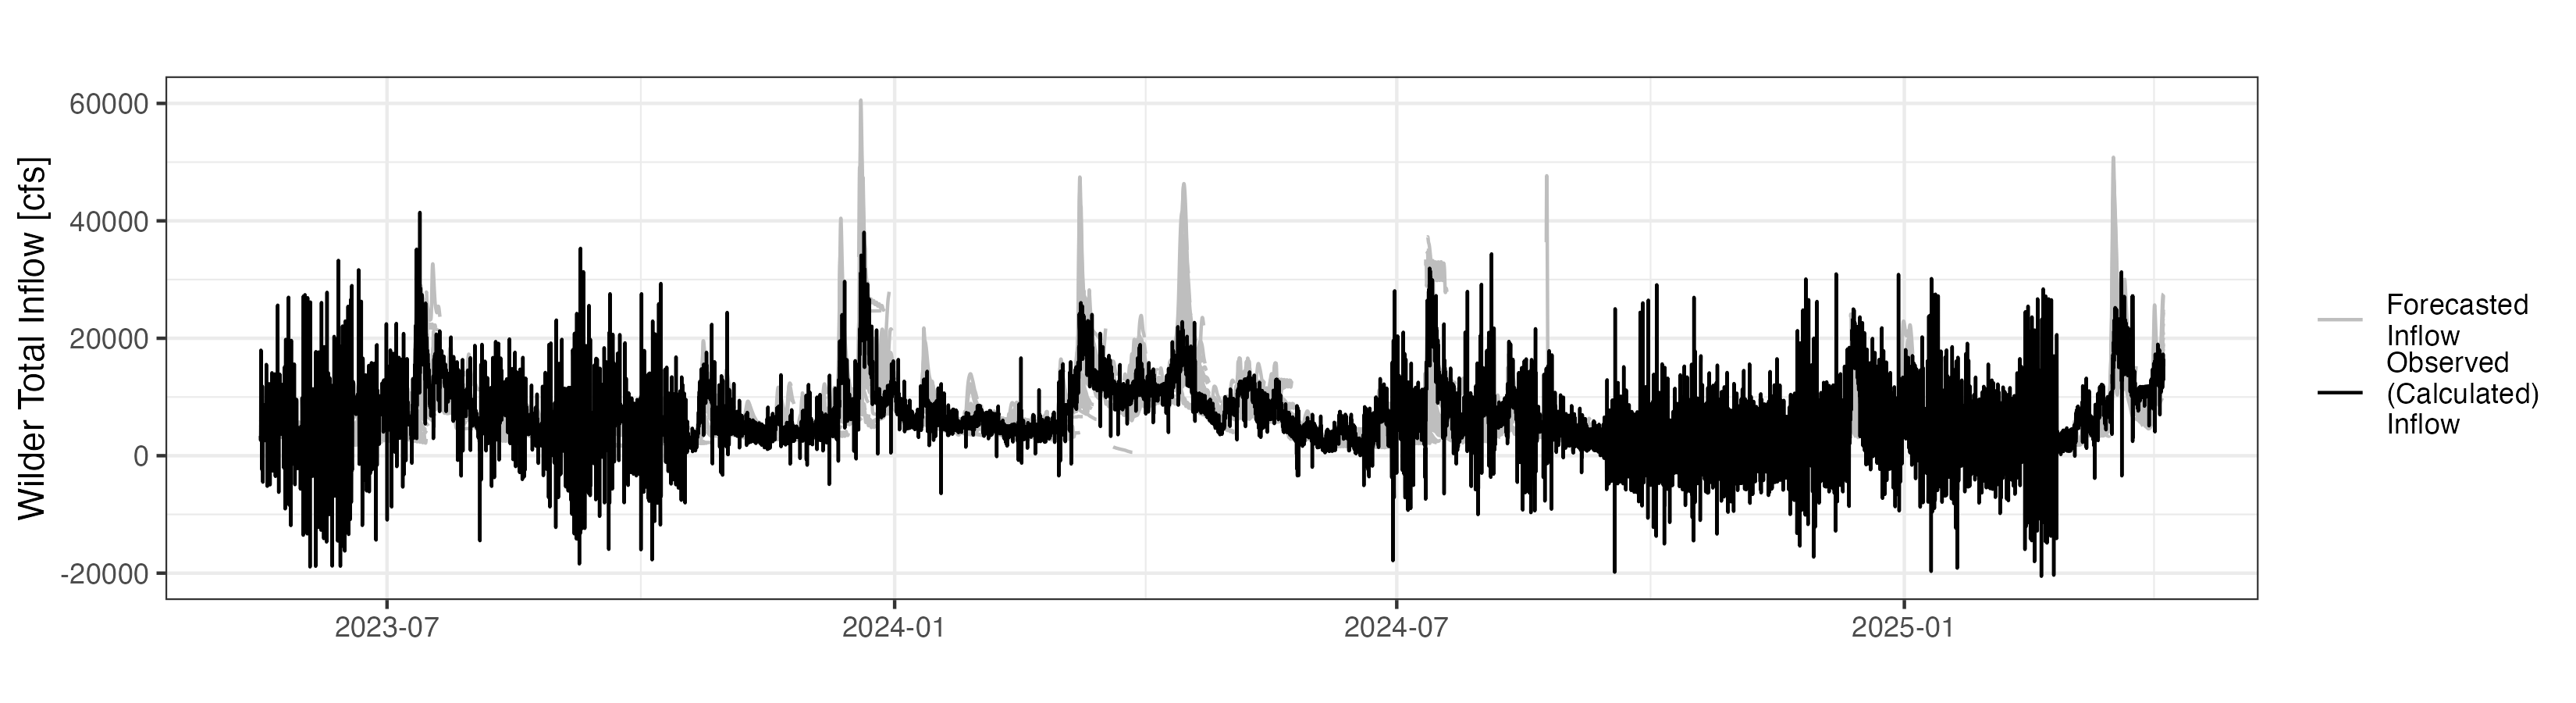
\includegraphics[width=\linewidth]{1a-wilder_0h.png}
%DIFDELCMD <     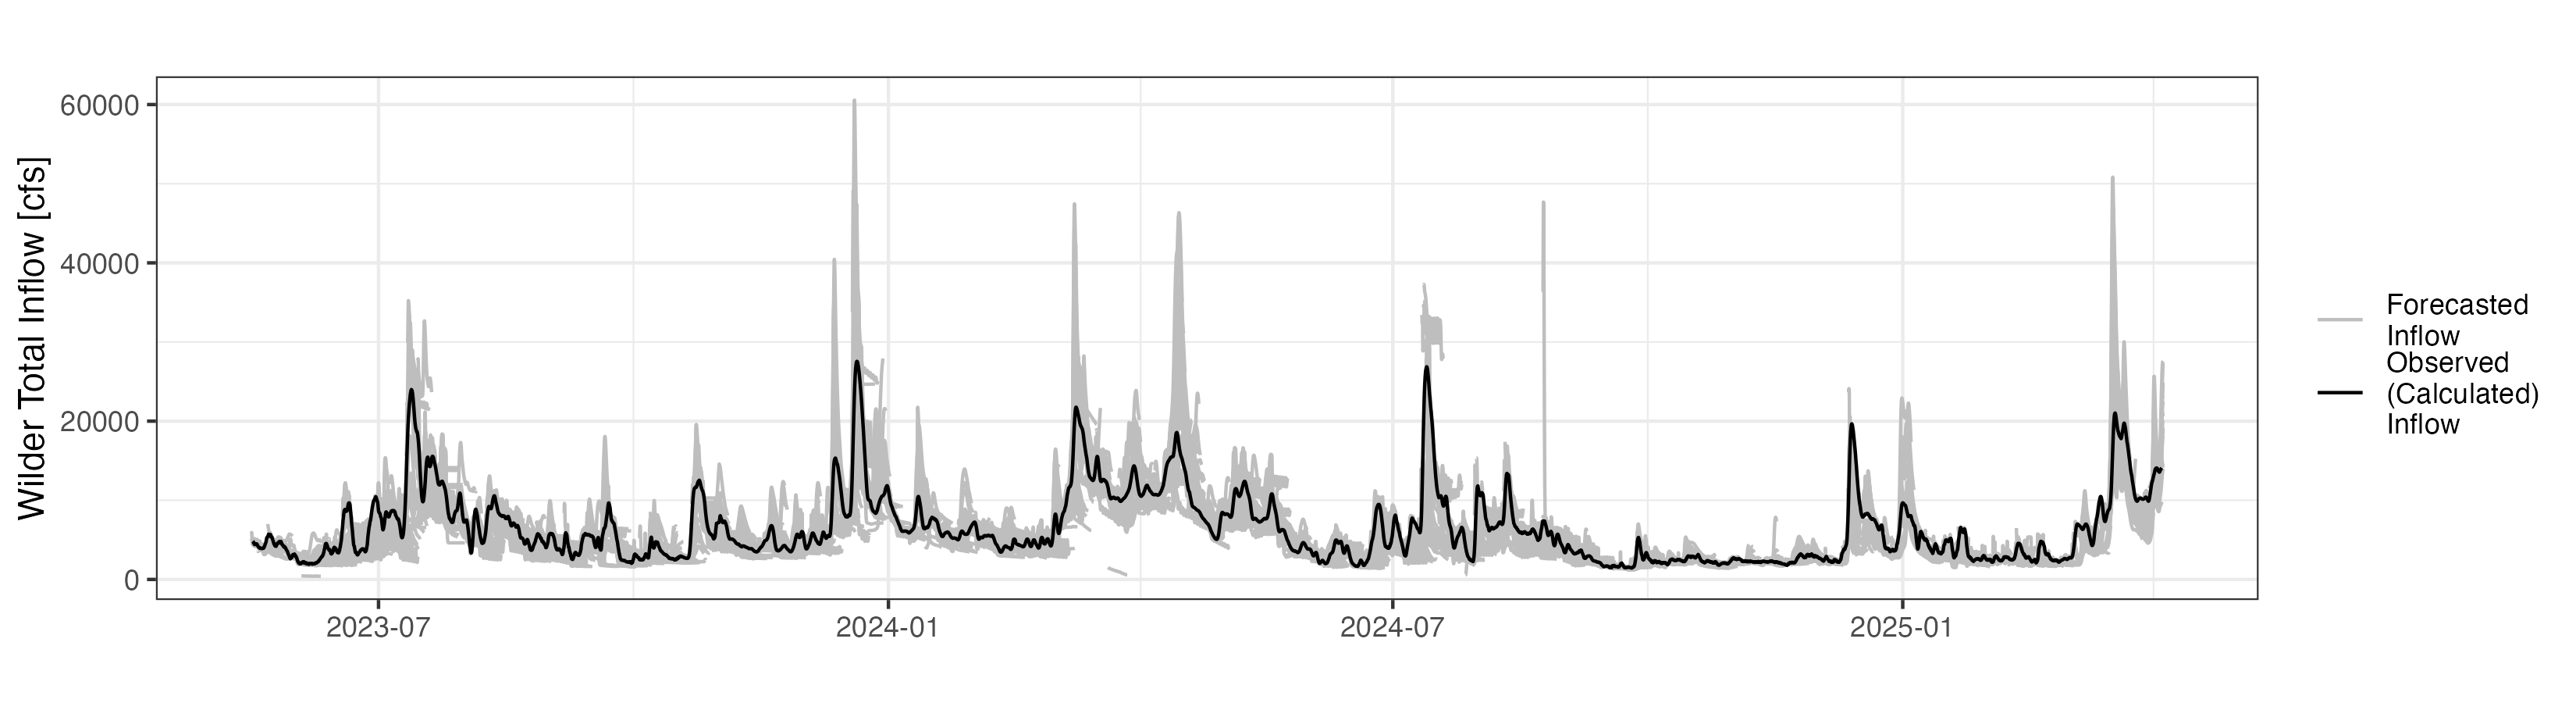
\includegraphics[width=\linewidth]{1b-wilder_24h.png}
%DIFDELCMD <     %%%
%DIFDELCMD < \caption{%
{%DIFAUXCMD
\DIFdelFL{The top figure shows the unsmoothed inflow and bottom figure shows the smoothed inflow used in the evaluation. The black lines show the calculated inflow based on forebay observations and dam outflow and the gray lines show the forecasts for reference.}}
    %DIFAUXCMD
%DIFDELCMD < \label{fig:smoothing}
%DIFDELCMD < \end{figure}
%DIFDELCMD < 

%DIFDELCMD < %%%
\DIFdelend %iv)	Traditional evaluation metrics
\subsection{Traditional inflow evaluation metrics}

Traditional deterministic forecast evaluation metrics that are particularly relevant to inflow forecasting include measures of average behavior, correlation, and bias. Additional metrics include higher order moments of the forecast distributions, categorical forecast performance, and conditional statistics \citep{st-aubinPrecisionReliabilityForecasts2022, hewamalageForecastEvaluationData2023}. This section is not intended to be a comprehensive review of deterministic forecast evaluation metrics. Therefore, we recommend some simple metrics which can be augmented as needed for particular applications. These metrics should be computed for a variety of lead times as well as seasonally to fully assess forecast performance across a range of conditions. 

Average hydrologic forecast behavior is typically measured with an error metric such as root mean squared error (RMSE), Nash-Sutcliffe Efficiency (NSE) \DIFdelbegin \DIFdel{, or King-Gupta }\DIFdelend \DIFaddbegin \DIFadd{\mbox{%DIFAUXCMD
\citep{nashRiverFlowForecasting1970}}\hskip0pt%DIFAUXCMD
, or Kling-Gupta }\DIFaddend Efficiency (KGE) \DIFdelbegin \DIFdel{(refs)}\DIFdelend \DIFaddbegin \DIFadd{\mbox{%DIFAUXCMD
\citep{guptaDecompositionMeanSquared2009}}\hskip0pt%DIFAUXCMD
}\DIFaddend . We recommend KGE because it \DIFdelbegin \DIFdel{is not skewed by large values where }\DIFdelend \DIFaddbegin \DIFadd{decomposes forecast performance into correlation, a variability ratio, and a bias ratio, so that a low score can be attributed to a specific deficiency rather than only registered as large aggregate error. }\DIFaddend NSE and RMSE \DIFdelbegin \DIFdel{are due to the use of a squared error term}\DIFdelend \DIFaddbegin \DIFadd{aggregate squared error into a single number, which makes them more strongly influenced by the largest errors and less diagnostic about their source}\DIFaddend . The KGE is given by

\begin{equation}
    \text{KGE}=1-\sqrt{(r-1)^2+\left(\frac{\sigma_f}{\sigma_o}-1\right)^2+\left(\frac{\mu_f}{\mu_o}-1\right)^2}
\end{equation}
where $r$ is the linear correlation coefficient, $\sigma_f$ is the standard deviation of the forecast, $\sigma_o$ is the standard deviation of the observations, $\mu_f$ is the mean of the forecast, and $\mu_o$ is the mean of the observations. Values of KGE that are greater than \DIFdelbegin \DIFdel{-0.41 }\DIFdelend \DIFaddbegin \DIFadd{$-0.41$ }\DIFaddend are better than \DIFaddbegin \DIFadd{using }\DIFaddend the mean of the observations \DIFaddbegin \DIFadd{as a predictor \mbox{%DIFAUXCMD
\citep{knobenTechnicalNoteInherent2019a}}\hskip0pt%DIFAUXCMD
}\DIFaddend , but larger values are preferred up to the maximum value of 1 for a perfect forecast. \DIFdelbegin \DIFdel{We note that }\DIFdelend \DIFaddbegin \DIFadd{Because this threshold is not zero, }\DIFaddend NSE and KGE have different properties and \DIFdelbegin \DIFdel{so }\DIFdelend should not be used interchangeably\DIFdelbegin \DIFdel{\mbox{%DIFAUXCMD
\citep{knobenTechnicalNoteInherent2019a}}\hskip0pt%DIFAUXCMD
. }\DIFdelend \DIFaddbegin \DIFadd{, and intuition built on NSE values does not transfer to KGE. The two metrics answer different questions and we recommend reporting both: KGE to diagnose where a forecast is deficient, and, as described below, a skill score against an explicit benchmark to compare a forecast against a meaningful alternative and across locations.
}\DIFaddend 

The \DIFdelbegin \DIFdel{bias }\DIFdelend \DIFaddbegin \DIFadd{error, or residual, }\DIFaddend of a single forecast \DIFdelbegin \DIFdel{point }\DIFdelend is the difference between \DIFdelbegin \DIFdel{observed and forecasted values but this may be expressed as a percentage }\DIFdelend \DIFaddbegin \DIFadd{the forecast and the observation. Bias is the systematic component of error, the tendency of a forecast to be too high or too low on average, and is conventionally expressed }\DIFaddend for a set of forecasts \DIFdelbegin \DIFdel{by averaging across all bias values 
}\DIFdelend \DIFaddbegin \DIFadd{as a percentage of total observed volume
}\DIFaddend 

\begin{equation}
    \text{PBIAS} = 100\ [\%]\times\frac{\sum(f_i-o_i)}{\sum(o_i)}
\end{equation}

where $\text{PBIAS}$ measures the tendency of a forecast ($f$) to be greater than (positive values) or less than (negative values) than observations ($o$). 

Correlation measures the strength of a linear relationship between observations and forecasts is computed using the Pearson correlation coefficient

\begin{equation}
    r = \DIFdelbegin \DIFdel{\frac{\sum(o_i-\mu_o)(f_i-\mu_f)}{\sqrt{\sum(o_i-\mu_o)^2(f_i-\mu_f)^2}}
}\DIFdelend \DIFaddbegin \DIFadd{\frac{\sum(o_i-\mu_o)(f_i-\mu_f)}{\sqrt{\sum(o_i-\mu_o)^2\ \sum(f_i-\mu_f)^2}}
}\DIFaddend \end{equation}

where $r$ can range from -1 to 1 but for forecast evaluation, negative values would indicate poor forecast performance.

\DIFaddbegin \DIFadd{For any of these metrics, skill score versions can be computed which are useful when comparing forecast quality between sites with different statistical properties (see Section \ref{sec:benchmarks}). A skill score compares one forecast to another reference forecast using a certain metric. The NSE is the natural starting point, because the NSE is already a skill score: it measures the forecast against the mean of the observations. Replacing that reference with an explicit benchmark forecast gives
}

\begin{equation}\DIFadd{\label{eq:nsess}
    \text{NSE}_{SS}= \frac{\text{NSE}_{f}-\text{NSE}_{ref}}{1-\text{NSE}_{ref}} = 1-\frac{\text{MSE}_{f}}{\text{MSE}_{ref}}
}\end{equation}

\DIFadd{where $\text{NSE}_{f}$ is the metric for the forecast being evaluated, $\text{NSE}_{ref}$ is the same metric computed for the reference forecast, $\text{MSE}$ is mean squared error, and $\text{NSE}_{SS}$ is the NSE skill score. The second equality shows what the score measures directly: the fraction of the reference forecast's squared error that the forecast under evaluation eliminates. A skill score has a maximum value of 1 when the forecast is perfect, is 0 when the forecast performs no better than the reference, and is negative when it performs worse. The reference forecast is often taken to be the persistence forecast, climatology, or some other existing forecast. The same construction applies to any of the metrics above, KGE included, but the NSE version has the advantage that it is interpretable as a proportional reduction in squared error and that it makes explicit what reference a raw NSE value is implicitly using.
}

\subsection{\DIFadd{Extension to probabilistic and ensemble forecasts}}\label{sec:probabilistic}

\DIFadd{The framework described above is agnostic to whether the forecast being evaluated is deterministic or probabilistic. Probabilistic forecasts are valuable for assessing the risk associated with certain operational decisions, which is particularly useful for compliance or market related concerns. Our evaluation framework can be used with either probabilistic or deterministic forecasts. The main difference being in the choice of metrics and visualizations, the overall process remains the same. Where ensemble or probabilistic products are available, metrics such as the continuous ranked probability score (CRPS) can be used. CRPS has the useful property that it reduces to mean absolute error (MAE) for a deterministic forecast, so the two can be compared on a common scale. Diagrams such as rank histograms and reliability diagrams are useful for assessing properties of ensemble forecasts. 
}


\DIFaddend \section{Case Study: Great River Hydro}

Great River Hydro \DIFaddbegin \DIFadd{(GRH) }\DIFaddend is New England’s largest conventional hydropower generator. As a private, independent power producer, GRH owns and operates 589 megawatts of \DIFdelbegin \DIFdel{nominal hydropower capacity }\DIFdelend \DIFaddbegin \DIFadd{installed nameplate hydropower capacity across 13 generating stations on the Connecticut and Deerfield Rivers }\DIFaddend in ISO New England. In this evaluation we focused on the inflow to three main hydropower producing dams in the system, Wilder, Bellows Falls, and Vernon (Figure \ref{fig:map}) as well as three main tributaries, the Ottauquechee, Sugar and White Rivers.

\DIFaddbegin \DIFadd{The three dams lie in series on the main stem of the Connecticut River, with Wilder upstream, followed by Bellows Falls, then Vernon. The three projects are operated jointly, so releases from each become inflow to the next. The only significant local flows occur between Wilder and Bellows Falls in the form of the three tributaries mentioned above. These three sites were selected from the larger set shown in Figure \ref{fig:map} because they are the largest generators on the system and they are where the operators concentrate their scheduling attention. In addition, these projects are part of an ongoing relicensing process through the Federal Energy Regulatory Commission (FERC), which includes new limits to forebay fluctuations. The remaining facilities in Figure \ref{fig:map} are smaller and are not covered by the same license conditions.
}

\DIFadd{Basin hydrology is snowmelt influenced, with a spring freshet typically spanning March through May, convective rainfall in summer, and rain and rain-on-snow driven events in winter. Several tributaries have upstream flood control regulation by the U.S. Army Corps of Engineers, which contributes to inflow variability that is not directly weather driven.
}

\begin{table}[ht]
\centering
\caption{\DIFaddFL{Physical characteristics of the six evaluation points. Drainage areas are from the USGS National Water Information System for the reference gage listed. Mainstem areas are nested, so the area above Vernon includes those above Bellows Falls and Wilder.}}\label{tab:basin}
\begin{tabular}{lllrr}
  \hline
\DIFaddFL{Location }& \DIFaddFL{Type }& \DIFaddFL{USGS reference gage }& \DIFaddFL{Area (mi$^2$) }& \DIFaddFL{Area (km$^2$) }\\
  \hline
\DIFaddFL{Wilder             }& \DIFaddFL{Mainstem dam }& \DIFaddFL{01144500 West Lebanon, NH   }& \DIFaddFL{4,092 }& \DIFaddFL{10,598 }\\
\DIFaddFL{Bellows Falls      }& \DIFaddFL{Mainstem dam }& \DIFaddFL{01154500 North Walpole, NH  }& \DIFaddFL{5,493 }& \DIFaddFL{14,227 }\\
\DIFaddFL{Vernon             }& \DIFaddFL{Mainstem dam }& \DIFaddFL{01156500 Vernon, VT         }& \DIFaddFL{6,266 }& \DIFaddFL{16,229 }\\
\DIFaddFL{White River        }& \DIFaddFL{Tributary    }& \DIFaddFL{01144000 West Hartford, VT  }&   \DIFaddFL{690 }&  \DIFaddFL{1,787 }\\
\DIFaddFL{Sugar River        }& \DIFaddFL{Tributary    }& \DIFaddFL{01152500 West Claremont, NH }&   \DIFaddFL{269 }&    \DIFaddFL{697 }\\
\DIFaddFL{Ottauquechee River }& \DIFaddFL{Tributary    }& \DIFaddFL{01151500 North Hartland, VT }&   \DIFaddFL{221 }&    \DIFaddFL{572 }\\
   \hline
\end{tabular}
\end{table}

\subsection{\DIFadd{Operating context}}\label{sec:context}

\DIFadd{The three dams have limited storage relative to their inflow and are operated as run-of-river facilities. Their daily cycle consists of an upward ramp, a period of flexible generation, a downward ramp, and a refill period. Generation is bid into the ISO New England day-ahead market, so the day-ahead inflow volume is the quantity that matters most to the operators, since it sets what they can bid into the market. The binding operational constraint comes from the FERC relicensing of the three lower Connecticut River dams, which imposed a $\pm$0.5 foot ($\approx$15 cm) limit on forebay fluctuation, with penalties for exceedance. The central operating problem is therefore committing generation based on an uncertain inflow forecast without violating the forebay limits. This is what motivated the cumulative-error and threshold-exceedance metrics in Section \ref{sec:tailored}.
}

\DIFadd{At the time of the evaluation the operators used an in-house forecast built from National Weather Service River Forecast Center forecasts, routed to the dam locations and adjusted using operator judgment. This is the incumbent product against which the two commercial forecasts were evaluated, and it is labeled GRH in the results.
}

\DIFaddend Setting up a \DIFdelbegin \DIFdel{real time }\DIFdelend \DIFaddbegin \DIFadd{real-time }\DIFaddend evaluation required the development of an automated data platform that enabled sharing of \DIFdelbegin \DIFdel{real time }\DIFdelend \DIFaddbegin \DIFadd{real-time }\DIFaddend system data as well as the forecasts. This was necessary to share certain data with external parties for the purposes of forecast evaluation. While such a system may not be necessary for evaluations conducted internally by a single organization, some form of data access (API, database, etc.) is required for a \DIFdelbegin \DIFdel{real time }\DIFdelend \DIFaddbegin \DIFadd{real-time }\DIFaddend forecast evaluation. Such systems incur an up-front cost that should be considered when deciding on an evaluation approach. In addition, \DIFdelbegin \DIFdel{real time }\DIFdelend \DIFaddbegin \DIFadd{real-time }\DIFaddend evaluations come with all of the challenges of any operational system, such as system uptime, latency\DIFaddbegin \DIFadd{, }\DIFaddend and maintenance. \DIFaddbegin \DIFadd{These factors may help decide if a forecast is viable before any evaluation is done; a forecast that cannot be produced operationally should not be considered in a real-time evaluation.
}\DIFaddend 

%<I believe that a lot of the effort was for GRH to set up the real time feed from the participants/candidate products? should there be some info here? It is somewhat important because the standard business model has been for operators to perform their own forecasts. And nnow the business model is changing. And the incumbent product is well set up with knowledgebsle staff. So the new product needs to be not only better to change decisions AND be accessible logistically - the pooint being that new products need to work on:
%- accuracy skill
%- cost of deployment
%- ease of procurement
%- consistency when data/platforms goes down - what are the plans B
%> All of those are necessary and the motivation for a real time benchmark. Also - does that mean that you have stats beyond the accuracy skills? how many time systems were off etc. While those may not be shared, this is important academically for staff to realize what real time is. >

\begin{figure}
    \centering
    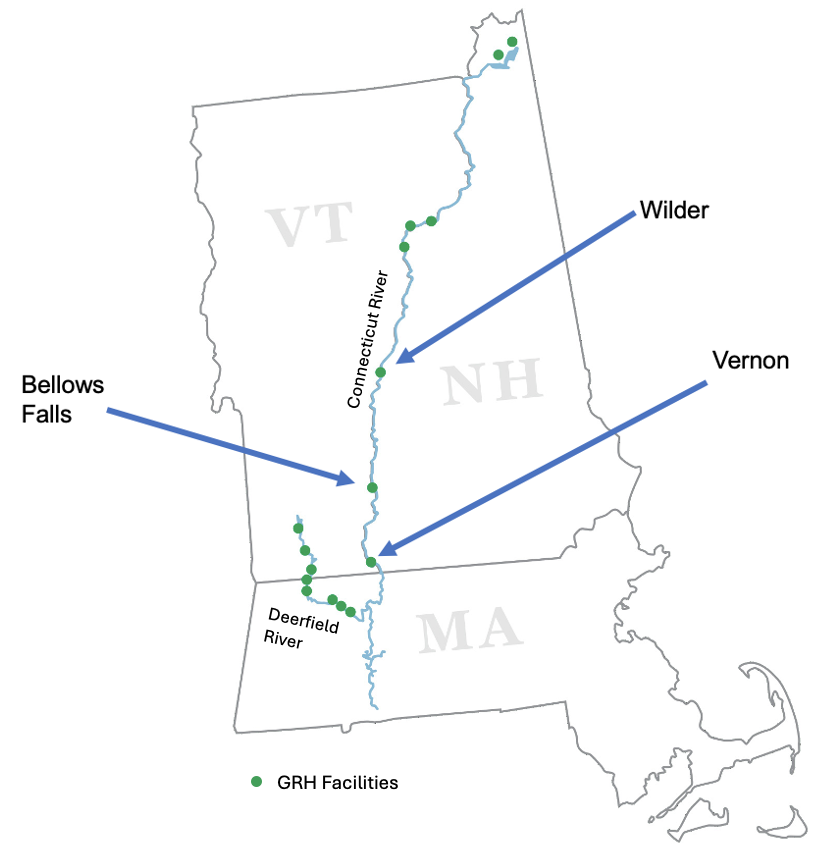
\includegraphics[width=0.5\linewidth]{2-map2.png}
    \caption{The Great River Hydro system in the Northeast U.S. with the locations of the three major dams in this evaluation.}
    \label{fig:map}
\end{figure}

We ran the \DIFdelbegin \DIFdel{real time }\DIFdelend \DIFaddbegin \DIFadd{real-time }\DIFaddend evaluation for almost \DIFdelbegin \DIFdel{2 yearsfrom July }\DIFdelend \DIFaddbegin \DIFadd{two years, from June }\DIFaddend 2023 to \DIFdelbegin \DIFdel{May }\DIFdelend \DIFaddbegin \DIFadd{April }\DIFaddend 2025\DIFaddbegin \DIFadd{, }\DIFaddend with regular feedback from the operators. We evaluated two commercial forecast products which are anonymized and labeled as A and B. In addition we evaluated the GRH in-house forecast which is a combination of RFC forecasts, routing, and operator judgment. During the initial few months of the evaluation we focused on generic metrics of forecast performance. As the quantity of data increased we transitioned to seasonally computed metrics and tailored metrics developed in collaboration with the system operators.

\DIFaddbegin \DIFadd{The three products differ in the coverage they provided over this period, which constrains how they can be compared. Forecast B was available for the full period, giving 657 day-ahead forecasts at each dam. Forecast A was discontinued in November 2024 and the in-house forecast archive also ends in November 2024, giving 539 and 528 day-ahead forecasts respectively. The three products overlap on 510 days at each dam, from 3 June 2023 to 20 November 2024. Metrics computed over each product's full available record, which is what we report, are therefore not computed over identical samples. We repeated the calculation restricted to the 510 common days and the ranking of the three products is unchanged at all three dams, with individual metrics shifting by no more than 0.03 NSE, so we report the full-record values so as not to discard any data. This kind of partial coverage reflects the operational realities of any real-time evaluation.
}

\subsection{\DIFadd{Forecast products}}\label{sec:products}

\DIFadd{Anonymization of the commercial products limits reproducibility, so we describe each to the extent our agreements allow. Forecast A is produced by a consulting firm using a conceptual rainfall-runoff model with hydraulic routing through the Connecticut River main stem, driven by a commercial numerical weather prediction forecast, and issued once daily at an hourly timestep out to roughly 8 days. Forecast B is produced by a technology firm using a machine learning model trained on gauge and remotely sensed catchment observations, issued twice daily at hourly timestep out to 10 days. The GRH in-house forecast combines RFC forecasts with routing and operator judgment and extends only through the day-ahead period, roughly 32 hours, because that is the horizon it is used for. Neither vendor released model internals or calibration and validation diagnostics, and we did not have access to them. A utility evaluating commercial forecast products generally cannot inspect them and must judge them on operational performance, which is part of the motivation for this framework. A full procurement evaluation should also weigh the operational cost, data dependencies, and ease of integration of each product alongside its skill, since these differ substantially between the two commercial products evaluated here.
}

\subsection{\DIFadd{Hydrology of the evaluation period}}\label{sec:period}

\DIFadd{The evaluation period included the July 2023 Vermont flood. This event produced the largest calculated inflows of the evaluation at Vernon (83,100 cfs, 2,353 m$^3$/s) and Bellows Falls (67,000 cfs). A December 2023 rain-on-snow event produced the largest inflow at Wilder (27,600 cfs) and the second largest at Vernon and Bellows Falls. The evaluation period also included spring freshets of 2024 and 2025 and dry summer conditions in both 2023 and 2024. The period therefore sampled a reasonable range of the conditions relevant to GRH operations. It did not, however, sample the full distribution of hydrologic conditions. Notably, the July 2023 event produced one of the ten largest flows ever recorded on the main stem of the Connecticut River. The evaluation also did not include any severe multi-year drought. Any real-time evaluation is bounded in this way, and the conclusions below should be taken as conditional on the observed period. 
}

\DIFaddend While most weather driven inflow forecasts are available hourly for the next 7-10 days, the volumetric forecast for the next day is the most important for GRH. This largely sets what they can bid into the \DIFdelbegin \DIFdel{day ahead }\DIFdelend \DIFaddbegin \DIFadd{day-ahead }\DIFaddend market. Table \ref{tab:metrics} \DIFdelbegin \DIFdel{) show }\DIFdelend \DIFaddbegin \DIFadd{shows }\DIFaddend the overall forecast evaluation metrics for the two commercial forecasts (A, B), the GRH in-house forecast (GRH), and the benchmark\DIFdelbegin \DIFdel{s}\DIFdelend  perfect and persistence forecasts for the one-day-ahead forecasts. Overall we found that for this time period, GRH's in-house forecast was roughly similar to forecast B but better than forecast A\DIFdelbegin \DIFdel{overall}\DIFdelend . This overall tabular view is a good way to get quick comparisons between forecasts but can obfuscate certain forecast behaviors, especially seasonal.

%DIF <  latex table generated in R 4.5.1 by xtable 1.8-4 package
%DIF <  Thu Jul 31 14:54:43 2025
\DIFaddbegin \DIFadd{Table \ref{tab:metrics} also illustrates the cross-location comparability problem noted in Section \ref{sec:benchmarks}. Based on NSE alone, forecast A appears to perform best at Vernon (0.81), followed by Wilder (0.72), and worst at Bellows Falls (0.55), which invites the conclusion that Bellows Falls is where the forecast most needs improvement. That conclusion is an artifact of the metric. NSE is normalized by the variance of the observations, and regulated flows tend to have less variability than natural flows, so inflows subject to more regulation tend to produce higher NSE values for the same quality of forecast. The persistence forecast makes the effect visible: its NSE is $-0.81$ at Wilder, 0.39 at Bellows Falls, and 0.80 at Vernon, tracking the increasing regulation further downstream. Said another way, simply carrying forward the previous day's inflow already explains most of the variance at Vernon, so there is little room left for a forecast to improve on it, whereas at Wilder the same benchmark is far worse than the observed mean.
}

\DIFadd{Because NSE is itself a skill score against the mean of the observations (Section \ref{sec:benchmarks}), the fix is to change the reference rather than the metric. The NSE skill score of Equation \ref{eq:nsess} computed against persistence (denoted NSE$_{SS}$ in Table \ref{tab:metrics}) is comparable across locations, and it inverts the apparent ordering. Forecast A is strongest at Wilder (0.85), not weakest, and at Vernon it scores 0.03, meaning it reduces the squared error of a persistence forecast by three percent. The product with the highest raw NSE of the three sites is therefore the one adding almost nothing to what an operator could obtain by assuming today's inflow will repeat. At Bellows Falls, where the raw NSE was lowest, forecast A retains a modest 0.25. The other two products hold real skill at all three sites, 0.91 and 0.94 at Wilder, 0.85 and 0.77 at Bellows Falls, and 0.44 and 0.47 at Vernon for forecast B and the in-house forecast respectively; the two are close enough at Vernon that they should be treated as comparable there. Restricting the calculation to the 510 days common to all three products leaves this picture intact, with forecast A at Vernon falling slightly below persistence ($-0.01$). This example shows how interpretations based on a single metric can lead to potentially erroneous conclusions and underscores the importance of using multiple metrics in any evaluation, especially when comparing forecasts between locations.
}

\DIFaddend \begin{table}[ht]
\centering
\caption{\DIFdelbeginFL \DIFdelFL{Overall }\DIFdelendFL \DIFaddbeginFL \DIFaddFL{Day-ahead }\DIFaddendFL forecast evaluation metrics for the \DIFdelbeginFL \DIFdelFL{real time }\DIFdelendFL \DIFaddbeginFL \DIFaddFL{real-time }\DIFaddendFL evaluation conducted from \DIFdelbeginFL \DIFdelFL{July }\DIFdelendFL \DIFaddbeginFL \DIFaddFL{June }\DIFaddendFL 2023 to \DIFdelbeginFL \DIFdelFL{May }\DIFdelendFL \DIFaddbeginFL \DIFaddFL{April }\DIFaddendFL 2025\DIFaddbeginFL \DIFaddFL{, }\DIFaddendFL for the two commercial forecasts (A, B), the GRH in-house forecast (GRH), and the \DIFdelbeginFL \DIFdelFL{benchmarks }\DIFdelendFL \DIFaddbeginFL \DIFaddFL{benchmark }\DIFaddendFL perfect and persistence forecasts. \DIFaddbeginFL \DIFaddFL{$n$ is the number of day-ahead forecasts evaluated; the three products cover different portions of the period, as described above. NSE$_{SS}$ is the NSE skill score of Equation \ref{eq:nsess} computed with the persistence forecast as the reference, which unlike NSE and KGE is directly comparable across locations. It is computed from unrounded metrics and can be recovered from the RMSE column as $1-(\text{RMSE}_{f}/\text{RMSE}_{ref})^2$.}\DIFaddendFL }\label{tab:metrics}
\DIFdelbeginFL %DIFDELCMD < \begin{tabular}{llrrrr}
%DIFDELCMD <   %%%
\DIFdelendFL \DIFaddbeginFL \begin{tabular}{llrrrrrrr}
  \DIFaddendFL \hline
\DIFaddbeginFL \DIFaddFL{Location }& \DIFaddendFL Forecast         & \DIFdelbeginFL \DIFdelFL{Location }\DIFdelendFL \DIFaddbeginFL \DIFaddFL{$n$ }\DIFaddendFL &   NSE   & KGE  & PBIAS \DIFaddbeginFL \DIFaddFL{(\%) }\DIFaddendFL & \DIFdelbeginFL \DIFdelFL{r }\DIFdelendFL \DIFaddbeginFL \DIFaddFL{RMSE (cfs) }& \DIFaddFL{$r$ }& \DIFaddFL{NSE$_{SS}$ }\DIFaddendFL \\
  \hline
\DIFaddbeginFL \DIFaddFL{Wilder        }& \DIFaddendFL A           & \DIFdelbeginFL \DIFdelFL{Wilder     }\DIFdelendFL \DIFaddbeginFL \DIFaddFL{539 }\DIFaddendFL &  0.72   & 0.83 &  \DIFdelbeginFL \DIFdelFL{-8.00    }\DIFdelendFL \DIFaddbeginFL \DIFaddFL{$-8.0$ }\DIFaddendFL & \DIFaddbeginFL \DIFaddFL{2,278 }& \DIFaddendFL 0.88 \DIFaddbeginFL & \DIFaddFL{0.85 }\DIFaddendFL \\
              \DIFaddbeginFL & \DIFaddendFL B           & \DIFdelbeginFL \DIFdelFL{Wilder     }\DIFdelendFL \DIFaddbeginFL \DIFaddFL{657 }\DIFaddendFL &  0.83   & 0.88 &    \DIFdelbeginFL \DIFdelFL{0.10     }\DIFdelendFL \DIFaddbeginFL \DIFaddFL{0.1  }\DIFaddendFL & \DIFaddbeginFL \DIFaddFL{1,786 }& \DIFaddendFL 0.93 \DIFaddbeginFL & \DIFaddFL{0.91 }\DIFaddendFL \\
              \DIFaddbeginFL & \DIFaddendFL GRH         & \DIFdelbeginFL \DIFdelFL{Wilder     }\DIFdelendFL \DIFaddbeginFL \DIFaddFL{528 }\DIFaddendFL &  0.88   & 0.89 &  \DIFdelbeginFL \DIFdelFL{-9.90    }\DIFdelendFL \DIFaddbeginFL \DIFaddFL{$-9.9$ }\DIFaddendFL & \DIFaddbeginFL \DIFaddFL{1,476 }& \DIFaddendFL 0.95 \DIFaddbeginFL & \DIFaddFL{0.94 }\DIFaddendFL \\
              \DIFaddbeginFL & \DIFaddendFL perfect     & \DIFdelbeginFL \DIFdelFL{Wilder     }\DIFdelendFL \DIFaddbeginFL \DIFaddFL{657 }\DIFaddendFL &  1.00   & 1.00 &    \DIFdelbeginFL \DIFdelFL{0.00     }\DIFdelendFL \DIFaddbeginFL \DIFaddFL{0.0  }\DIFaddendFL &     \DIFaddbeginFL \DIFaddFL{0 }& \DIFaddendFL 1.00 \DIFaddbeginFL & \DIFaddFL{1.00 }\DIFaddendFL \\
              \DIFaddbeginFL & \DIFaddendFL persistence & \DIFdelbeginFL \DIFdelFL{Wilder     }\DIFdelendFL \DIFaddbeginFL \DIFaddFL{657 }\DIFaddendFL & \DIFdelbeginFL \DIFdelFL{-0.81 }\DIFdelendFL \DIFaddbeginFL \DIFaddFL{$-0.81$ }\DIFaddendFL & 0.02 & \DIFdelbeginFL \DIFdelFL{-75.90   }\DIFdelendFL \DIFaddbeginFL \DIFaddFL{$-75.9$ }\DIFaddendFL & \DIFaddbeginFL \DIFaddFL{5,866 }& \DIFaddendFL 0.75 \DIFaddbeginFL & \DIFaddFL{0.00 }\DIFaddendFL \\
\DIFaddbeginFL \DIFaddFL{Bellows Falls }& \DIFaddendFL A           & \DIFdelbeginFL \DIFdelFL{Bellows    }\DIFdelendFL \DIFaddbeginFL \DIFaddFL{539 }\DIFaddendFL &  0.55   & 0.77 &    \DIFdelbeginFL \DIFdelFL{0.40     }\DIFdelendFL \DIFaddbeginFL \DIFaddFL{0.4  }\DIFaddendFL & \DIFaddbeginFL \DIFaddFL{5,904 }& \DIFaddendFL 0.77 \DIFaddbeginFL & \DIFaddFL{0.25 }\DIFaddendFL \\
              \DIFaddbeginFL & \DIFaddendFL B           & \DIFdelbeginFL \DIFdelFL{Bellows    }\DIFdelendFL \DIFaddbeginFL \DIFaddFL{657 }\DIFaddendFL &  0.91   & 0.95 &    \DIFdelbeginFL \DIFdelFL{0.60     }\DIFdelendFL \DIFaddbeginFL \DIFaddFL{0.6  }\DIFaddendFL & \DIFaddbeginFL \DIFaddFL{2,615 }& \DIFaddendFL 0.95 \DIFaddbeginFL & \DIFaddFL{0.85 }\DIFaddendFL \\
              \DIFaddbeginFL & \DIFaddendFL GRH         & \DIFdelbeginFL \DIFdelFL{Bellows    }\DIFdelendFL \DIFaddbeginFL \DIFaddFL{528 }\DIFaddendFL &  0.85   & 0.88 & \DIFdelbeginFL \DIFdelFL{-10.40   }\DIFdelendFL \DIFaddbeginFL \DIFaddFL{$-10.4$ }\DIFaddendFL & \DIFaddbeginFL \DIFaddFL{3,309 }& \DIFaddendFL 0.93 \DIFaddbeginFL & \DIFaddFL{0.77 }\DIFaddendFL \\
              \DIFaddbeginFL & \DIFaddendFL perfect     & \DIFdelbeginFL \DIFdelFL{Bellows    }\DIFdelendFL \DIFaddbeginFL \DIFaddFL{657 }\DIFaddendFL &  1.00   & 1.00 &    \DIFdelbeginFL \DIFdelFL{0.00     }\DIFdelendFL \DIFaddbeginFL \DIFaddFL{0.0  }\DIFaddendFL &     \DIFaddbeginFL \DIFaddFL{0 }& \DIFaddendFL 1.00 \DIFaddbeginFL & \DIFaddFL{1.00 }\DIFaddendFL \\
              \DIFaddbeginFL & \DIFaddendFL persistence & \DIFdelbeginFL \DIFdelFL{Bellows    }\DIFdelendFL \DIFaddbeginFL \DIFaddFL{657 }\DIFaddendFL &  0.39   & 0.35 & \DIFdelbeginFL \DIFdelFL{-39.20   }\DIFdelendFL \DIFaddbeginFL \DIFaddFL{$-39.2$ }\DIFaddendFL & \DIFaddbeginFL \DIFaddFL{6,831 }& \DIFaddendFL 0.87 \DIFaddbeginFL & \DIFaddFL{0.00 }\DIFaddendFL \\
\DIFaddbeginFL \DIFaddFL{Vernon        }& \DIFaddendFL A           & \DIFdelbeginFL \DIFdelFL{Vernon     }\DIFdelendFL \DIFaddbeginFL \DIFaddFL{539 }\DIFaddendFL &  0.81   & 0.83 & \DIFdelbeginFL \DIFdelFL{-11.30   }\DIFdelendFL \DIFaddbeginFL \DIFaddFL{$-11.3$ }\DIFaddendFL & \DIFaddbeginFL \DIFaddFL{5,097 }& \DIFaddendFL 0.91 \DIFaddbeginFL & \DIFaddFL{0.03 }\DIFaddendFL \\
              \DIFaddbeginFL & \DIFaddendFL B           & \DIFdelbeginFL \DIFdelFL{Vernon     }\DIFdelendFL \DIFaddbeginFL \DIFaddFL{657 }\DIFaddendFL &  0.89   & 0.94 &    \DIFdelbeginFL \DIFdelFL{1.70     }\DIFdelendFL \DIFaddbeginFL \DIFaddFL{1.7  }\DIFaddendFL & \DIFaddbeginFL \DIFaddFL{3,872 }& \DIFaddendFL 0.94 \DIFaddbeginFL & \DIFaddFL{0.44 }\DIFaddendFL \\
              \DIFaddbeginFL & \DIFaddendFL GRH         & \DIFdelbeginFL \DIFdelFL{Vernon     }\DIFdelendFL \DIFaddbeginFL \DIFaddFL{528 }\DIFaddendFL &  0.89   & 0.88 & \DIFdelbeginFL \DIFdelFL{-11.00   }\DIFdelendFL \DIFaddbeginFL \DIFaddFL{$-11.0$ }\DIFaddendFL & \DIFaddbeginFL \DIFaddFL{3,764 }& \DIFaddendFL 0.95 \DIFaddbeginFL & \DIFaddFL{0.47 }\DIFaddendFL \\
              \DIFaddbeginFL & \DIFaddendFL perfect     & \DIFdelbeginFL \DIFdelFL{Vernon     }\DIFdelendFL \DIFaddbeginFL \DIFaddFL{657 }\DIFaddendFL &  1.00   & 1.00 &    \DIFdelbeginFL \DIFdelFL{0.00     }\DIFdelendFL \DIFaddbeginFL \DIFaddFL{0.0  }\DIFaddendFL &     \DIFaddbeginFL \DIFaddFL{0 }& \DIFaddendFL 1.00 \DIFaddbeginFL & \DIFaddFL{1.00 }\DIFaddendFL \\
              \DIFaddbeginFL & \DIFaddendFL persistence & \DIFdelbeginFL \DIFdelFL{Vernon     }\DIFdelendFL \DIFaddbeginFL \DIFaddFL{657 }\DIFaddendFL &  0.80   & 0.69 & \DIFdelbeginFL \DIFdelFL{-18.10   }\DIFdelendFL \DIFaddbeginFL \DIFaddFL{$-18.1$ }\DIFaddendFL & \DIFaddbeginFL \DIFaddFL{5,167 }& \DIFaddendFL 0.93 \DIFaddbeginFL & \DIFaddFL{0.00 }\DIFaddendFL \\
   \hline
\end{tabular}
\end{table}

Figure \ref{fig:fc-lead-time} shows the performance of all the available forecasts and benchmarks out to a 10 day lead time. The GRH in-house forecast is only used to develop bids for the \DIFdelbegin \DIFdel{day ahead }\DIFdelend \DIFaddbegin \DIFadd{day-ahead }\DIFaddend market so it does not extend the full 10 day period. At Wilder and Vernon all three forecasts perform roughly similar with 1-3 days of lead time with the A and B forecasts diverging after that period. At Bellows Falls the three forecasts are \DIFaddbegin \DIFadd{more }\DIFaddend distinct in terms of quality with the B showing the best performance at most lead times followed by the GRH in-house forecast and then forecast A. \DIFdelbegin \DIFdel{Notably, after three days of }\DIFdelend \DIFaddbegin \DIFadd{Both commercial forecasts develop a growing negative bias with }\DIFaddend lead time, \DIFdelbegin \DIFdel{all forecasts exhibited some amount of bias at the downstream forecast locations which may be due to errors propagating from upstream}\DIFdelend \DIFaddbegin \DIFadd{and the bias grows further downstream, consistent with errors propagating through the cascading reservoirs. For forecast A, day-ahead PBIAS is 0.4\% at Bellows Falls and grows to $-19.1$\% by day 7; for forecast B the corresponding values are $-1.3$\% and $-7.8$\%. Because releases from each dam become inflow to the next, an error propagates directly to the next downstream project, and the effect compounds with lead time}\DIFaddend .

\begin{figure}
    \centering
    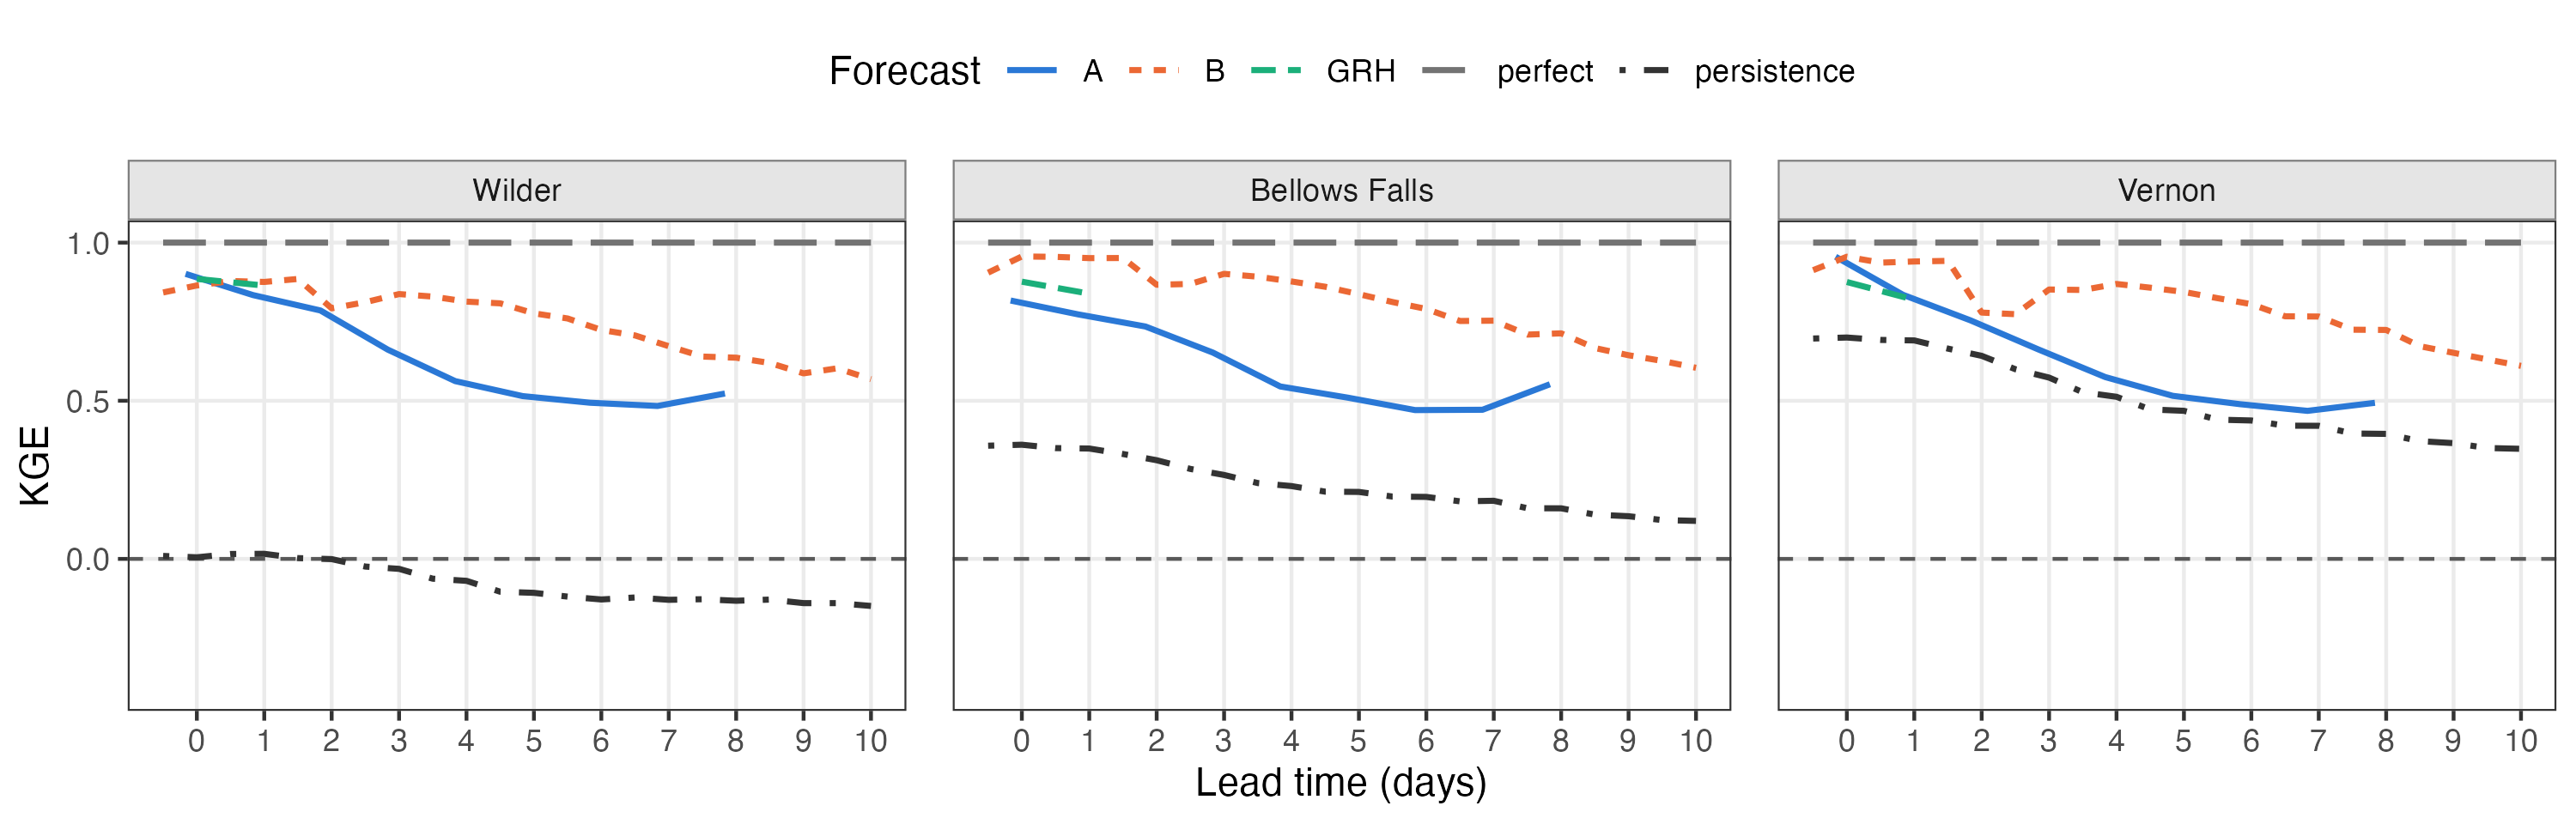
\includegraphics[width=.9\linewidth]{3a-daily-kge.png}
    
\includegraphics[width=.9\linewidth]{3b-daily-nse.png}
    
\includegraphics[width=.9\linewidth]{3c-daily-pbias.png}
    
\includegraphics[width=.9\linewidth]{3d-daily-r.png}
    \caption{Forecast performance metrics by lead time. A and B are commercial forecasts, GRH is an in-house forecast. The dashed line indicates the threshold where a forecast has no skill over the mean \DIFaddbeginFL \DIFaddFL{of the observations, which is NSE of 0 and KGE of $-0.41$}\DIFaddendFL . \DIFaddbeginFL \DIFaddFL{The persistence benchmark is a meaningful reference only over the first two days; beyond that it is shown for reference purposes only.}\DIFaddendFL }
    \label{fig:fc-lead-time}
\end{figure}

\DIFaddbegin \subsection{\DIFadd{Smoothing GRH calculated inflows}}\label{sec:smoothGRH}

\DIFadd{Figure \ref{fig:smoothing} shows an example of GRH hourly computed inflow data which has been smoothed using a triangular smoother. We used a 24-hour triangular window, implemented as two successive 24-hour moving averages of the hourly calculated inflow, which produces the triangular weighting. The window was matched to the operational timescale, in our application the day-ahead volumetric forecast is the quantity of interest, so smoothing at 24 hours removes sub-daily forebay noise without attenuating the daily signal being evaluated. Because the window directly affects the computed metrics, we repeated the day-ahead evaluation at window widths of 0 (no smoothing), 6, 12, and 24 hours (Table \ref{tab:smoothing}). Metrics improve slightly with increasing window width, as expected since smoothing removes observation noise, with the largest change being 0.05 NSE. Importantly, the ranking of the three products is unchanged at every window width at every location, and the gap between the two commercial products is stable: forecast B leads forecast A by 0.39 NSE at Bellows Falls with no smoothing and by 0.37 with 24-hour smoothing. The conclusions of the evaluation therefore do not depend on this choice. Evaluators should nonetheless state the window explicitly and check that their conclusions are insensitive to it, since a window wide enough to attenuate the signal of interest would flatter forecasts that under-predict variability. We recommend matching the window to the decision timescale rather than choosing the window that maximizes metric values.
}

\begin{figure}
    \centering
    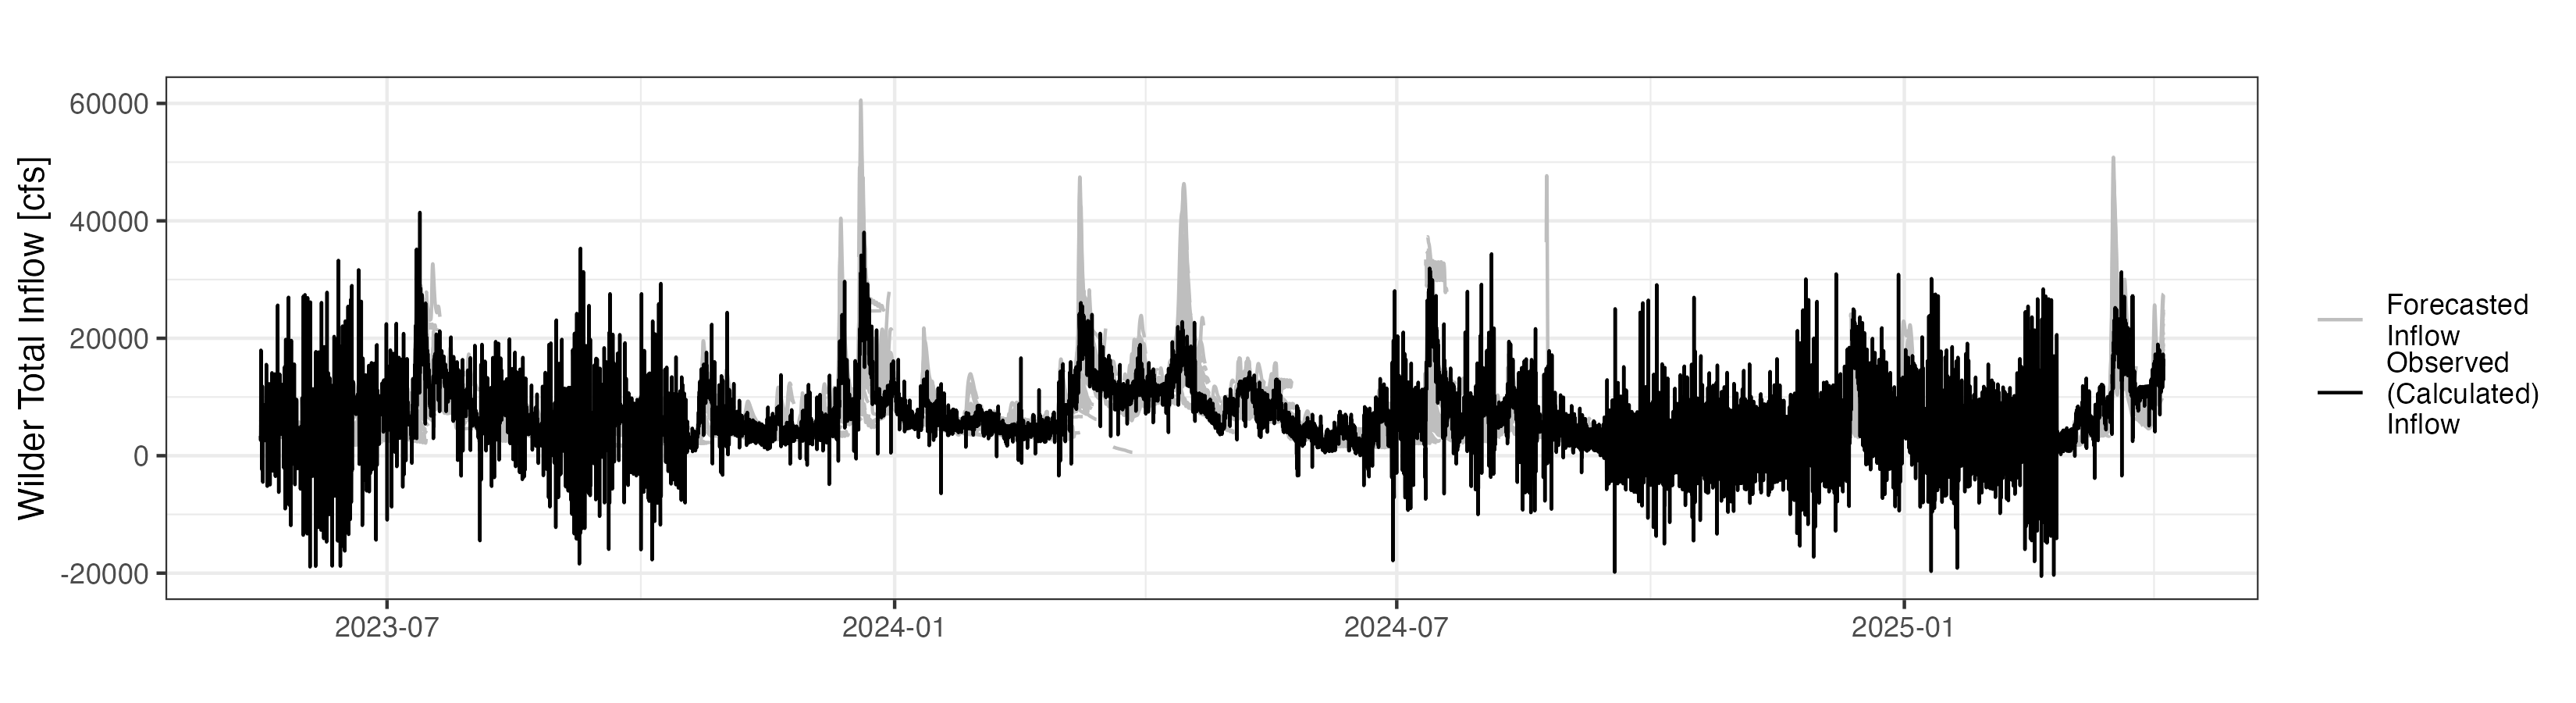
\includegraphics[width=\linewidth]{1a-wilder_0h.png}
    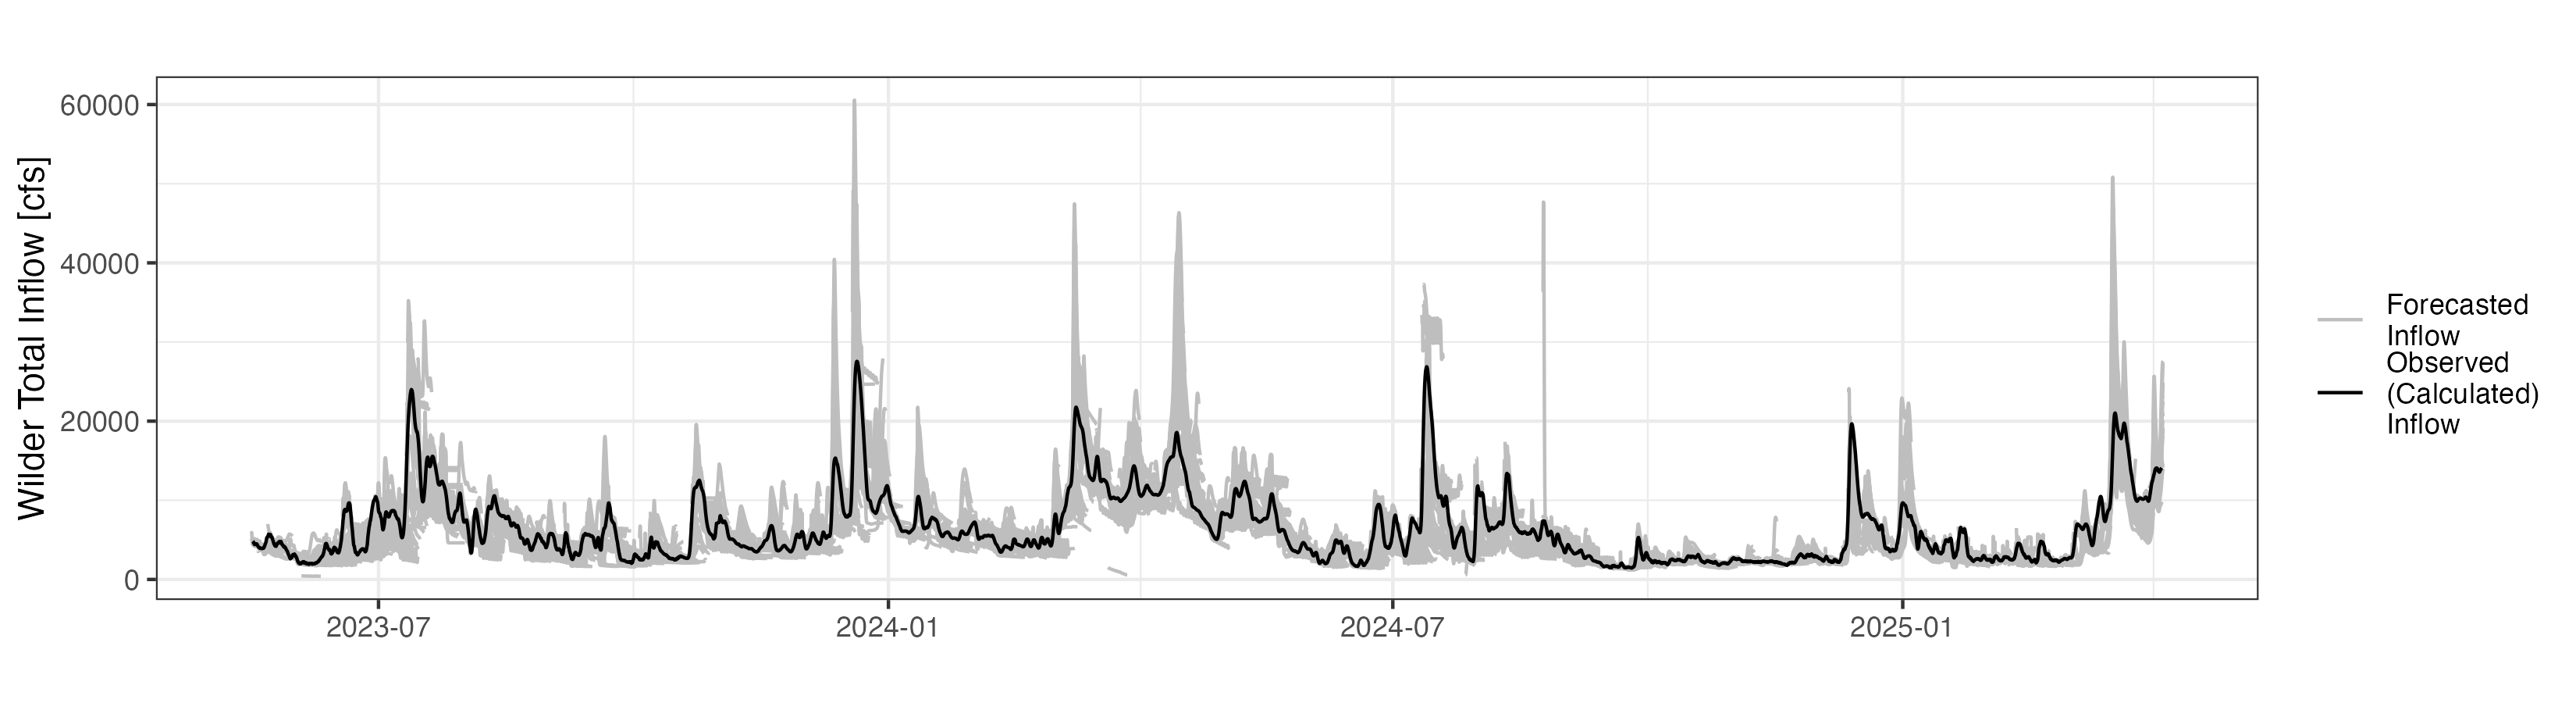
\includegraphics[width=\linewidth]{1b-wilder_24h.png}
    \caption{\DIFaddFL{Unsmoothed (top) and smoothed (bottom) calculated inflow at Wilder Dam, the latter being what was used in the evaluation. Black lines show the calculated inflow derived from forebay observations and dam outflow; gray lines show the forecasts for reference. Smoothing uses a 24-hour triangular window. Flows are in cubic feet per second (1,000 cfs $\approx$ 28.3 m$^3$/s).}}
    \label{fig:smoothing}
\end{figure}

\begin{table}[ht]
\centering
\caption{\DIFaddFL{Sensitivity of day-ahead NSE to the width of the triangular smoothing window applied to calculated inflow. The 24-hour column corresponds to the values reported in Table \ref{tab:metrics}. The ranking of the three forecasts is unchanged at every window width.}}\label{tab:smoothing}
\begin{tabular}{llrrrr}
  \hline
\DIFaddFL{Location }& \DIFaddFL{Forecast }& \DIFaddFL{0 h }& \DIFaddFL{6 h }& \DIFaddFL{12 h }& \DIFaddFL{24 h }\\
  \hline
\DIFaddFL{Wilder        }& \DIFaddFL{A   }& \DIFaddFL{0.70 }& \DIFaddFL{0.72 }& \DIFaddFL{0.72 }& \DIFaddFL{0.72 }\\
              & \DIFaddFL{B   }& \DIFaddFL{0.82 }& \DIFaddFL{0.83 }& \DIFaddFL{0.83 }& \DIFaddFL{0.83 }\\
              & \DIFaddFL{GRH }& \DIFaddFL{0.87 }& \DIFaddFL{0.87 }& \DIFaddFL{0.88 }& \DIFaddFL{0.88 }\\
\DIFaddFL{Bellows Falls }& \DIFaddFL{A   }& \DIFaddFL{0.50 }& \DIFaddFL{0.51 }& \DIFaddFL{0.52 }& \DIFaddFL{0.55 }\\
              & \DIFaddFL{B   }& \DIFaddFL{0.90 }& \DIFaddFL{0.90 }& \DIFaddFL{0.90 }& \DIFaddFL{0.91 }\\
              & \DIFaddFL{GRH }& \DIFaddFL{0.84 }& \DIFaddFL{0.83 }& \DIFaddFL{0.84 }& \DIFaddFL{0.85 }\\
\DIFaddFL{Vernon        }& \DIFaddFL{A   }& \DIFaddFL{0.79 }& \DIFaddFL{0.79 }& \DIFaddFL{0.79 }& \DIFaddFL{0.81 }\\
              & \DIFaddFL{B   }& \DIFaddFL{0.88 }& \DIFaddFL{0.88 }& \DIFaddFL{0.88 }& \DIFaddFL{0.89 }\\
              & \DIFaddFL{GRH }& \DIFaddFL{0.88 }& \DIFaddFL{0.88 }& \DIFaddFL{0.88 }& \DIFaddFL{0.89 }\\
   \hline
\end{tabular}
\end{table}

\subsection{\DIFadd{Seasonal performance}}\label{sec:seasonal}

\DIFaddend Figure \ref{fig:metrics-by-season} shows metrics by month for the entire evaluation period\DIFdelbegin \DIFdel{which reveals some trends }\DIFdelend \DIFaddbegin \DIFadd{, which reveals systematic variation }\DIFaddend in forecast quality \DIFdelbegin \DIFdel{in certain seasons. Namely forecasts tend to perform worse in the winter which is the wet season and worse in the summer which is the dry season . Forecasts tended to perform well during the snow melt season (April-July). The natural hydrology of the system is driven by different mechanisms in different seasons, for example, snow vs rain and baseflow vs direct runoff, which may explain the varying model performance by season}\DIFdelend \DIFaddbegin \DIFadd{by season. Skill is highest during the spring snowmelt period, roughly March through May, for all three products. It is lowest in late summer and fall for the commercial products, with A showing the sharpest degradation of any product in any season in January and February, where day-ahead KGE pooled across the three dams falls to 0.45 and $-0.67$ respectively, the latter below the plotted range. The seasons where performance is poorest are those in which inflow is driven by precipitation events: rain and rain-on-snow in winter and convective storms in summer. Both depend on precipitation forecasts which can be highly uncertain. Snowmelt-driven inflow is comparatively predictable because it is governed by an accumulated snowpack that can be observed in advance and melts over a period of weeks, so skill depends more on temperature, which is forecast more reliably than precipitation}\DIFaddend . Although forecast B tends to perform better overall, there are \DIFdelbegin \DIFdel{cases in which the A forecast }\DIFdelend \DIFaddbegin \DIFadd{months in which forecast A }\DIFaddend is better, \DIFaddbegin \DIFadd{notably April and May, }\DIFaddend highlighting the difficulty of selecting a single deterministic forecast.

\begin{figure}
    \centering
    
\includegraphics[width=.9\linewidth]{4a-da-month-kge.png}
    
\includegraphics[width=.9\linewidth]{4b-da-month-nse.png}
    
\includegraphics[width=.9\linewidth]{4c-da-month-pbias.png}
    
\includegraphics[width=.9\linewidth]{4d-da-month-r.png}
    \caption{Forecast performance metrics by month. A and B are commercial forecasts, GRH is an in-house forecast. The dashed line indicates the threshold where a forecast has no skill over the mean \DIFaddbeginFL \DIFaddFL{of the observations, which is NSE of 0 and KGE of $-0.41$}\DIFaddendFL .}
    \label{fig:metrics-by-season}
\end{figure}





\subsection{Tailored metrics}\DIFaddbegin \label{sec:tailored}
\DIFaddend 

In addition to the generic forecast evaluation metric\DIFaddbegin \DIFadd{s}\DIFaddend  described above, we developed several tailored metrics specifically relevant to the GRH system and its operations. \DIFaddbegin \DIFadd{Each arose from the feedback process described in steps 4 and 5 of Section \ref{sec:realtime}, and Table \ref{tab:tailored} traces each metric to the operator concern that prompted it. }\DIFaddend The first focused on \DIFdelbegin \DIFdel{day ahead }\DIFdelend \DIFaddbegin \DIFadd{day-ahead }\DIFaddend forecast performance as shown in the previous section. This was motivated by the \DIFdelbegin \DIFdel{day ahead }\DIFdelend \DIFaddbegin \DIFadd{day-ahead }\DIFaddend market that GRH bids into, as such they focus their attention heavily on the 1-2 day ahead period where the forecasts matter the most. Operationally, they adjust their flows \DIFdelbegin \DIFdel{after this point}\DIFdelend \DIFaddbegin \DIFadd{daily}\DIFaddend , so no forecast is used after the 2 day mark.

\DIFdelbegin \DIFdel{During the Federal Energy Regulatory Commission (FERC ) }\DIFdelend \DIFaddbegin \begin{table}[ht]
\centering
\caption{\DIFaddFL{Tailored metrics developed during the evaluation, the operator concern that prompted each, and the approximate point in the evaluation at which it was added. Metric development converged within roughly the first six months.}}\label{tab:tailored}
\begin{tabular}{p{0.26\linewidth}p{0.42\linewidth}p{0.20\linewidth}}
  \hline
\DIFaddFL{Metric }& \DIFaddFL{Operator concern }& \DIFaddFL{Added }\\
  \hline
\DIFaddFL{Day-ahead volumetric skill }& \DIFaddFL{Day-ahead market bids are set from next-day inflow volume, not hourly shape }& \DIFaddFL{Months 1--2 }\\
\DIFaddFL{Seasonal metric breakdown }& \DIFaddFL{Products were suspected to behave differently in snowmelt and rain driven regimes }& \DIFaddFL{Months 3--4 }\\
\DIFaddFL{Cumulative forebay error }& \DIFaddFL{Average error does not indicate whether the forebay band would be breached }& \DIFaddFL{Months 4--6 }\\
\DIFaddFL{Forebay exceedance probability from a non-neutral start }& \DIFaddFL{Operators rarely begin a day at the center of a forebay band, this more accurately represents the risk of exceeding the limit on the second day }& \DIFaddFL{Months 5--6 }\\
   \hline
\end{tabular}
\end{table}

\DIFadd{As described in Section \ref{sec:context}, the FERC }\DIFaddend relicensing for the three main dams on the lower Connecticut \DIFdelbegin \DIFdel{river a strict limit on forebay fluctuations was imposed . GRH was given a +/- }\DIFdelend \DIFaddbegin \DIFadd{River imposed a $\pm$}\DIFaddend 0.5 foot \DIFdelbegin \DIFdel{operating range after which penalties are incurred}\DIFdelend \DIFaddbegin \DIFadd{($\approx$15 cm) limit on forebay fluctuation, with penalties for exceedance}\DIFaddend . Given GRH\DIFdelbegin \DIFdel{’}\DIFdelend \DIFaddbegin \DIFadd{'}\DIFaddend s reliance on the inflow forecast, a metric was developed that captures the chance of the forebay limit being exceeded if the inflow forecast is used directly. Figure \ref{fig:cum-error} shows where the forebay would be after a certain amount of time if the forecast was used directly to set a \DIFdelbegin \DIFdel{pass inflow }\DIFdelend \DIFaddbegin \DIFadd{pass-inflow }\DIFaddend condition (i.e., inflow=outflow). The error bars extend to the 2.5th and 97.5th percentile of all forecasts. We can see that rarely would a forecast cause the forebay to exceed the 0.5 foot limit during the first day of operations, after which the operators can adjust. \DIFaddbegin \DIFadd{We note that the pass-inflow assumption is not how the system is actually operated. In practice operators schedule generation to a market bid, which typically means departing from inflow during the day and recovering the forebay overnight. The metric is idealized and intended to be an upper limit on the compliance risk a forecast carries rather than a prediction of observed exceedance rates. Capturing the actual risk of exceedance given a certain operation requires a scheduling model with direct operator oversight, which is discussed in Section \ref{sec:discussion}.
}\DIFaddend 

\begin{figure}
    \centering
    
\includegraphics[width=1\linewidth]{5-cum-error-5pct.png}
    \caption{\DIFdelbeginFL \DIFdelFL{The cumulative probability of exceeding a 0.5 foot operating range }\DIFdelendFL \DIFaddbeginFL \DIFaddFL{Cumulative forebay error by lead time }\DIFaddendFL if \DIFdelbeginFL \DIFdelFL{the }\DIFdelendFL operations were set to pass inflow (inflow=outflow)\DIFaddbeginFL \DIFaddFL{, }\DIFaddendFL where inflow was determined by \DIFdelbeginFL \DIFdelFL{the various }\DIFdelendFL \DIFaddbeginFL \DIFaddFL{each }\DIFaddendFL inflow \DIFaddbeginFL \DIFaddFL{forecast. Points show the median across all }\DIFaddendFL forecasts \DIFaddbeginFL \DIFaddFL{and error bars span the 2.5th to 97.5th percentile}\DIFaddendFL . \DIFaddbeginFL \DIFaddFL{Dashed lines mark the $\pm$0.5 foot ($\approx$15 cm) FERC compliance band.}\DIFaddendFL }
    \label{fig:cum-error}
\end{figure}

Figure \ref{fig:prob-exeed-threshold} (top) shows the corresponding probability of exceeding the 0.5 foot limit given a neutral forebay starting position on day 0. Results suggest that chances of exceedance are \DIFdelbegin \DIFdel{less than }\DIFdelend \DIFaddbegin \DIFadd{below }\DIFaddend 10\% for all forecasts \DIFdelbegin \DIFdel{for }\DIFdelend \DIFaddbegin \DIFadd{at }\DIFaddend all lead times in the 1-3 day range\DIFaddbegin \DIFadd{, with the highest values being 5.9\% for forecast A at Bellows Falls on day 1 and 6.0\% at Vernon on day 3. On this basis the products are difficult to distinguish}\DIFaddend . GRH was also interested in \DIFdelbegin \DIFdel{seeing a more realistic situation involving a non-optimal }\DIFdelend \DIFaddbegin \DIFadd{the more demanding and more common situation of a non-neutral }\DIFaddend forebay starting position on the second day, \DIFdelbegin \DIFdel{what was the probability of exceeding the 0.5 foot range, which is }\DIFdelend shown in Figure \ref{fig:prob-exeed-threshold} (bottom). \DIFdelbegin \DIFdel{We can see that }\DIFdelend \DIFaddbegin \DIFadd{Here }\DIFaddend the probabilities are \DIFdelbegin \DIFdel{much higher , up to 25\% in some cases for the A forecast}\DIFdelend \DIFaddbegin \DIFadd{substantially higher and the products separate clearly: at Bellows Falls, forecast A reaches 23.7\% on day 1 and 11.9\% on day 2, against 1.8\% and 2.4\% for forecast B. At Vernon, forecast A reaches 10.1\% by day 3 against 5.2\% for forecast B}\DIFaddend . This information provides \DIFdelbegin \DIFdel{a detailed view of the }\DIFdelend \DIFaddbegin \DIFadd{another view of }\DIFaddend forecast performance that GRH can use to assess forecast quality.


\DIFaddbegin \DIFadd{The general point we would like to convey in this section is the importance of computing an array of traditional and tailored metrics. Hydrologic forecasts are highly complex and nuanced, and rarely will there be a cut and dry answer to which is better. Tailored metrics provide information to operators in ways that might be obscured by traditional evaluation metrics, ultimately providing more robust information for investment decisions.
}

\DIFaddend \begin{figure}
    \centering
     
\includegraphics[width=1\linewidth]{6a-threshold-1day.png}
    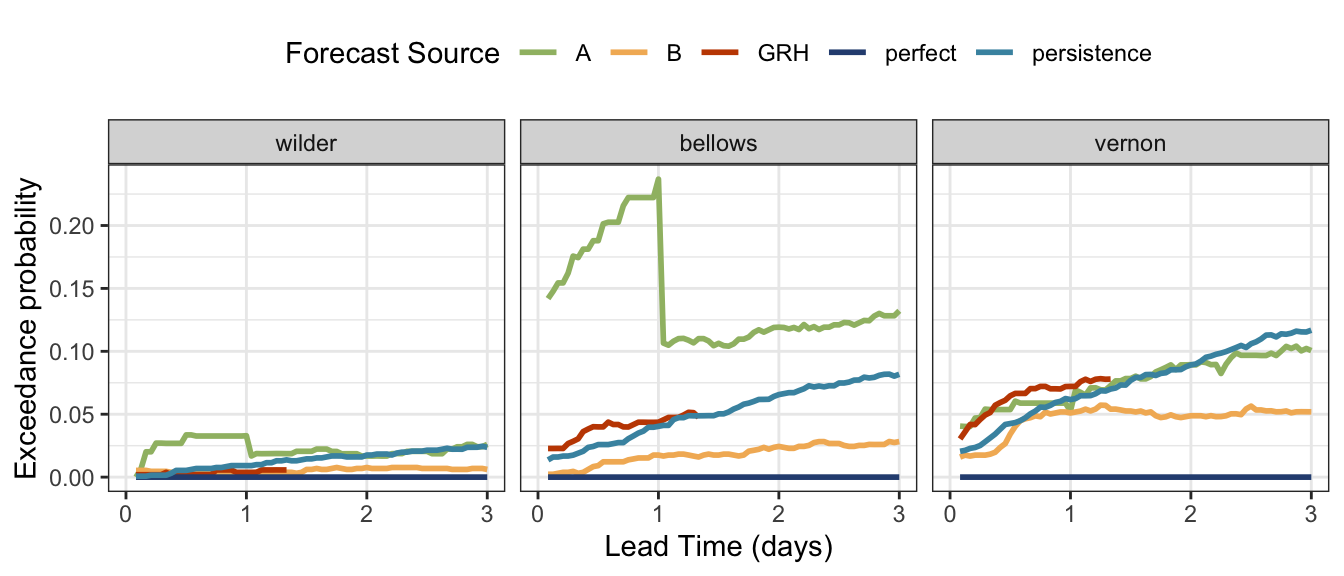
\includegraphics[width=1\linewidth]{6b-threshold-2day.png}
    \caption{Probability of exceeding \DIFdelbeginFL \DIFdelFL{a }\DIFdelendFL \DIFaddbeginFL \DIFaddFL{the $\pm$}\DIFaddendFL 0.5 foot \DIFaddbeginFL \DIFaddFL{($\approx$15 cm) forebay }\DIFaddendFL operating range \DIFaddbeginFL \DIFaddFL{under a pass-inflow assumption, }\DIFaddendFL given a neutral forebay starting position on day 0 (top)\DIFdelbeginFL \DIFdelFL{and probability of exceeding a 0.5 foot operating range on the second day}\DIFdelendFL , \DIFaddbeginFL \DIFaddFL{and }\DIFaddendFL given the forebay \DIFdelbeginFL \DIFdelFL{starting }\DIFdelendFL position \DIFaddbeginFL \DIFaddFL{carried over }\DIFaddendFL from the first day (bottom). \DIFaddbeginFL \DIFaddFL{The non-neutral start in the lower panel is the more common operating situation and separates the two commercial products, which the neutral start does not.}\DIFaddendFL }
    \label{fig:prob-exeed-threshold}
\end{figure}
%    \begin{figure}
%        \centering
%        \includegraphics[width=0.5\linewidth]{map3.png}
%        \caption{Enter Caption}
%        \label{fig:enter-label}
%    \end{figure}
%i)	Setting (Figure: map)
%v)	Development of tailored metrics
%vi)	Data visualizer (Figure)
%i)	Traditional metrics (graphs and table from visualizer)
%ii)	Tailored metrics 
%(1)	Tailored metrics

%\section{Results  (Cameron, Youngjun)}

%(2)	Tailored metric results

\section{Discussion}\DIFaddbegin \label{sec:discussion}
\DIFaddend %i)	Recommendation
%ii)	Value of the process
%iii)	Limitations

 In this paper we present a general framework that can be used in \DIFdelbegin \DIFdel{real time }\DIFdelend \DIFaddbegin \DIFadd{real-time }\DIFaddend (or near \DIFdelbegin \DIFdel{real time}\DIFdelend \DIFaddbegin \DIFadd{real-time}\DIFaddend ) for reservoir inflow forecast evaluation. \DIFdelbegin \DIFdel{The  evaluation can include }\DIFdelend \DIFaddbegin \DIFadd{Forecast products using AI/ML methods are being marketed to utilities at an increasing rate, and verification statistics supplied by vendors may not be verifiable. This framework is intended for that increasingly common situation where utilities are evaluating multiple forecasts, perhaps from multiple vendors, and hindcasting is not viable. The evaluation includes standard numerical }\DIFaddend forecast verification and validation but \DIFaddbegin \DIFadd{may }\DIFaddend also include other qualitative or specialized metrics of forecast quality. The framework calls for an iterative approach which involves direct operator feedback in the process. We also presented \DIFdelbegin \DIFdel{a successful }\DIFdelend \DIFaddbegin \DIFadd{an }\DIFaddend application of this evaluation framework to three reservoirs in the Great River Hydro system on the Connecticut River in the Northeast U.S. While there is no single evaluation approach that can apply to all forecasts, we present a range of options of both traditional and tailored metrics that will be suitable for many \DIFdelbegin \DIFdel{situations}\DIFdelend \DIFaddbegin \DIFadd{systems}\DIFaddend . The goal of \DIFdelbegin \DIFdel{such a }\DIFdelend \DIFaddbegin \DIFadd{this }\DIFaddend framework is to provide operators with information necessary for \DIFaddbegin \DIFadd{understanding the quality of existing forecasts and }\DIFaddend evaluating how much a particular forecast product \DIFdelbegin \DIFdel{will }\DIFdelend \DIFaddbegin \DIFadd{may }\DIFaddend improve their operations\DIFdelbegin \DIFdel{and ultimately }\DIFdelend \DIFaddbegin \DIFadd{. Ultimately this information can }\DIFaddend inform ongoing investment decisions (i.e. purchase external forecast products or improve existing internal forecast).

\DIFaddbegin \subsection{\DIFadd{Comparison with retrospective forecast evaluation}}

\DIFadd{Because the results presented here were all produced on an ongoing near real-time basis, it is reasonable to ask what a conventional retrospective evaluation might add. A retrospective evaluation provides larger sample sizes, a wider range of hydrologic conditions, and better coverage of hydrologic extremes since hindcasts can span decades where our evaluation spans less than two years. Hindcasts provide certainty in a forecast model's behavior for a wide range of historical conditions, although translating thousands of historical forecasts into operational decisions may be prohibitively expensive. In addition even if historical operations could be reconstructed for past conditions (such as with a scheduling optimization model), it is difficult or impossible to reconstruct the exact market conditions at the time of a decision. On the other hand, real-time evaluations can reflect exact operational conditions such as outages and market feedbacks, and requires no additional data or extra operator effort. We acknowledge that a real-time evaluation is not a replacement for retrospective verification and hindcast should be done where feasible. Where it is not, this framework provides a practical alternative.
}


\subsection{\DIFadd{From forecast quality to forecast value}}

\DIFadd{The metrics presented here are measures of forecast quality, not forecast value. Quality is a statistical property of a forecast paired with observational data. Value depends additionally on human decisions and the cost associated with forecast errors. A forecast can be more statistically accurate and yet carry less value, if the additional accuracy falls in a range where the operator would not act differently. We refer the reader to \mbox{%DIFAUXCMD
\cite{farkasEconomicValueWeather2025} }\hskip0pt%DIFAUXCMD
for a comprehensive review of the economic value of forecasts. 
}

\DIFadd{The tailored metrics in Section \ref{sec:tailored} are a step towards assessing forecast value. For example, the forebay exceedance probability is a quantity with a direct financial consequence, since exceedance incurs a penalty under the FERC license. This is a partial valuation, since it captures an upper limit on compliance risk but it is not put in terms of generation revenue. A more complete assessment of revenue requires a decision-support model which includes reservoir operations and market conditions. We recommend that operators treat a real-time quality evaluation as the first of two stages. The evaluation establishes which forecast products are plausibly worth adopting and produces the archive of forecasts that may be used to drive the second step where value is assessed.
}

\subsection{\DIFadd{Limitations and next steps}}

\DIFaddend In our \DIFdelbegin \DIFdel{real time evaluation of the }\DIFdelend \DIFaddbegin \DIFadd{real-time evaluation of the }\DIFaddend GRH inflow forecasts there was one commercial forecast that stood out as having better performance overall. However, it was not always the best in every month and every lead time. This underscores the difficulty of selecting a single best deterministic forecast. Moving to a probabilistic forecast may alleviate this somewhat but operators still need to bid \DIFdelbegin \DIFdel{in }\DIFdelend a fixed amount into energy markets so overall improvements in deterministic forecast skill are valuable.
\DIFaddbegin 

\DIFadd{A related lesson concerns how the numbers are reported rather than which forecast wins. Raw efficiency metrics implicitly measure a forecast against the mean of the observations, a reference that is easy to beat at some locations and hard to beat at others. Judged against persistence instead, one of the commercial products turned out to add almost nothing at the most regulated of the three sites, at the very location where its raw NSE was highest. An operator reading only the raw metrics would have drawn the opposite conclusion about where that product was performing well. We therefore recommend that any multi-site evaluation choose its benchmark deliberately and report skill relative to it, since this is the difference between knowing that a forecast explains most of the variance and knowing that it improves on the alternative the operator already has.
}

\DIFaddend In this study we did not address how much improvements in inflow forecasts will translate into improvements in hydropower operations and increased revenue. An important next step \DIFdelbegin \DIFdel{in this evaluation framework }\DIFdelend is to couple this evaluation with hydropower scheduling models to quantify increases in revenue from improved inflow forecasts. \DIFdelbegin \DIFdel{While this seems a straight forward next steps, many hydropower scheduling models work with ranges of operations that match the }\DIFdelend \DIFaddbegin \DIFadd{One difficulty in this approach is that scheduling models may be configured to reproduce a }\DIFaddend utility's \DIFdelbegin \DIFdel{bidding strategy and local market opportunities. This complexity implies that evaluating the opportunities for harnessing higher forecast accuracy may also requires updating scheduling models and exploring more monetized operations}\DIFdelend \DIFaddbegin \DIFadd{current bidding strategy, which was itself developed around the accuracy of its existing forecast. A more accurate forecast may show little revenue benefit simply because the model is not set up to exploit it. Quantifying the value of improved forecasts may therefore require revising the scheduling model and the operating strategy alongside any new forecast}\DIFaddend .

\DIFdelbegin \DIFdel{Real time }\DIFdelend \DIFaddbegin \DIFadd{Real-time }\DIFaddend forecast evaluations are inherently limited by the amount of time they are conducted. Ideally a forecast model's performance would be assessed over the full range of hydrologic conditions spanning multiple decades. \DIFdelbegin \DIFdel{A hindcast evaluation may account for the full range of hydrologic variability but this requires an operations model or considerable effort on the part of the system operators to re-operate the system for every hindcast . }\DIFdelend \DIFaddbegin \DIFadd{As described in Section \ref{sec:period}, our two-year period included a major regional flood and a significant rain-on-snow event. While the need for representing multiple high flow events is less important in the GRH system due to limited operational flexibility in these conditions, we also did not observe strong multi-year drought conditions. We therefore were not able to assess the quality of forecasts under highly water limited conditions. A hindcast evaluation would have provided a more comprehensive evaluation of forecast quality.
}

\DIFaddend The decision to pursue a \DIFdelbegin \DIFdel{real time or hindcast }\DIFdelend \DIFaddbegin \DIFadd{real-time or retrospective forecast }\DIFaddend evaluation must be made by the system operators \DIFdelbegin \DIFdel{depending }\DIFdelend \DIFaddbegin \DIFadd{based }\DIFaddend on their specific system needs and resource availability\DIFaddbegin \DIFadd{. We recommend a real-time evaluation be paired with a retrospective if both are feasible as they provide complementary views of forecast quality. We recommend that a real-time evaluation be conducted for a minimum of one year, although we acknowledge the industry preference may lean toward shorter evaluations, sometimes a single season. A single season samples only one hydrologic outcome, so the resulting assessment is conditional on the conditions that happened to occur.
}

\DIFadd{Two further limitations of the present evaluation should be noted. First, the calculated inflows against which we verify are derived from forebay elevation changes and dam outflow, so the observation record is itself a function of how the system was operated. This does not require a model to interpret, but it does mean the reference data is not independent of operations in the way a gauge record would be. Second, the three products did not cover identical portions of the evaluation period, as described in Section \ref{sec:context}, so the metrics in Table \ref{tab:metrics} are computed over overlapping periods but not identical sample sizes. We verified that restricting to the common period does not change the ranking so we opted for the largest sample size possible for each forecast so as to not discard any data}\DIFaddend . 

The iterative nature of this framework is perhaps its most valuable component. Having direct operator involvement and feedback helps to provide value to the operators. The development of tailored metrics make the results relevant to a particular system and helps with operator buy-in. Furthermore, both generic and tailored metrics can ultimately be extended to assess the impacts of inflow forecasts on hydropower scheduling. Particularly under dynamic electricity market conditions, evaluations of inflow forecasts can serve as key indicators for understanding how forecasting errors propagate through the system, influencing compliance with operational requirements, variations in actual power generation, and potential revenue for system operators. The analysis of inflow forecast performance, conducted in coordination with system operators, represents an important foundational step toward achieving these broader applications. In presenting this framework we hope to provide a template for further applications and unbiased evaluation of the myriad of inflow forecasts available to hydropower system operators.


\bmsection*{Data and Code}

Code for the evaluation is freely available
\footnote{https://github.com/HydroWIRES-PNNL/inflow-forecast-evaluation}. Sample data can be accessed from the data repository on Zenodo\footnote{https://doi.org/10.5281/zenodo.16921728}. 

Note that a pre-print non-peer reviewed draft of the manuscript has been uploaded to \url{https://eartharxiv.org/repository/view/10530/}. 

%\backmatter
\bmsection*{Author contributions}

Cameron Bracken - Conceptualization, Data Curation, Formal Analysis, Investigation, Methodology, Software, Validation, Visualization, Writing - Original Draft Preparation. Youngjun Son - Conceptualization, Data Curation, Formal Analysis, Investigation, Software, Validation, Visualization, Writing - Original Draft Preparation. Vince Tidwell - Conceptualization, Formal Analysis, Investigation, Methodology, Project Administration, Supervision, Writing - Original Draft Preparation. Nathalie Voisin -  Conceptualization, Methodology, Project Administration, Supervision, Funding Acquision, Writing – Original Draft.

%Conceptualization, Writing – Review & Editing, Formal Analysis, Investigation, Methodology
%Ideas; formulation or evolution of overarching research goals and aims.

%Data Curation
%Management activities to annotate (produce metadata), scrub data and maintain research data (including software code, where it is necessary for interpreting the data itself) for initial use and later reuse.

%Formal Analysis
%Application of statistical, mathematical, computational, or other formal techniques to analyze or synthesize study data.

%Funding Acquisition
%Acquisition of the financial support for the project leading to this publication.

%Investigation
%Conducting a research and investigation process, specifically performing the experiments, or data/evidence collection.

%Methodology
%Development or design of methodology; creation of models.

%Project Administration
%Management and coordination responsibility for the research activity planning and execution.

%Resources
%Provision of study materials, reagents, materials, patients, laboratory samples, animals, instrumentation, computing resources, or other analysis tools.

%Software
%Programming, software development; designing computer programs; implementation of the computer code and supporting algorithms; testing of existing code components.

%Supervision
%Oversight and leadership responsibility for the research activity planning and execution, including mentorship external to the core team.

%Validation
%Verification, whether as a part of the activity or separate, of the overall replication/reproducibility of results/experiments and other research outputs.

%Visualization
%Preparation, creation and/or presentation of the published work, specifically visualization/data presentation.

%Writing – Original Draft Preparation
%Creation and/or presentation of the published work, specifically writing the initial draft (including substantive translation).

%Writing – Review & Editing

%\bmsection*{Acknowledgments}


%\bmsection*{Financial disclosure}

%None reported.

\bmsection*{Conflict of interest}

The authors declare no potential conflict of interests.

\bibliography{GRH}


%\bmsection*{Supporting information}

%Additional supporting information may be found in the online version of the article at the publisher’s website.




%\appendix

%\bmsection{Program codes appear in Appendix\label{app1}}
%\vspace*{12pt}
%Using the package {\tt listings} you can add non-formatted text as you would do with \verb|\begin{verbatim}| but its main aim is to include the source code of any programming language within your document.\newline Use \verb|\begin{lstlisting}...\end{lstlisting}| for program codes without mathematics.

%The {\tt listings} package supports all the most common languages and it is highly customizable. If you just want to write code within your document, the package provides the {\tt lstlisting} environment; the output will be in Computer Modern typewriter font. Refer to the below example:


%\begin{lstlisting}[caption={Descriptive caption text},label=DescriptiveLabel, basicstyle=\fontsize{8}{10}\selectfont\ttfamily]
%for i:=maxint to 0 do
%begin
%{ do nothing }
%end;
%Write('Case insensitive ');
%WritE('Pascal keywords.');
%\end{lstlisting}



%\bmsubsection{Subsection title of first appendix\label{app1.1a}}

%\bmsubsubsection{Subsection title of first appendix\label{app1.1.1a}}

%\noindent\textbf{Unnumbered figure*}

%\nocite{*}% Show all bib entries - both cited and uncited; comment this line to view only cited bib entries;


%\bmsection*{Author Biography}

%\begin{biography}{\includegraphics[width=76pt,height=76pt,draft]{empty}}{
%{\textbf{Author Name.} Please check with the journal's author guidelines whether
%author biographies are required. They are usually only included for
%review-type articles, and typically require photos and brief
%biographies for each author.}}
%\end{biography}


\end{document}
